%%%%%%%%%%%%%%%%%%%%%%%%%%%%%%%%%%%%%%%%%%%%%%%%%%%%%%%%%%%
% EPFL report package, main thesis file
% Goal: provide formatting for theses and project reports
% Author: Mathias Payer <mathias.payer@epfl.ch>
%
% This work may be distributed and/or modified under the
% conditions of the LaTeX Project Public License, either version 1.3
% of this licen se or (at your option) any later version.
% The latest version of this license is in
%   http://www.latex-project.org/lppl.txt
%
%%%%%%%%%%%%%%%%%%%%%%%%%%%%%%%%%%%%%%%%%%%%%%%%%%%%%%%%%%%
\documentclass[a4paper,11pt,oneside]{report}
% Options: MScThesis, BScThesis, MScProject, BScProject
\usepackage[MScProject]{EPFLreport}
\usepackage{xspace}

% Additionnal packages
\usepackage{caption}
\usepackage{subcaption}
\usepackage{xcolor}

\title{Data corruption in plausibly deniable storage: challenges and potential solutions}
\author{Kilian d'Eternod}
\supervisor{Dr. Vero Estrada-Galiñanes}
\adviser{Prof. Bryan Ford}
%\coadviser{Second Adviser}
%\expert{The External Reviewer}

\newcommand{\sysname}{FooSystem\xspace}
\newcommand{\veg}[1]{\textcolor{purple}{VEG:#1}}

\begin{document}
\maketitle
%\makededication
\makeacks

\maketoc

%%%%%%%%%%%%%%%%%%%%%%
\chapter{Introduction}
%%%%%%%%%%%%%%%%%%%%%%

Plausible deniability is a powerful cryptographic primitive. In the context of data storage, it allows the user to hide sensitive information and deny their existence, which limits the coercion that can be applied on them.

It can be challenging to hide data while also keeping it consistent and protecting it against corruption. Often, the security guarantees renders this corruption unavoidable as the hidden data must be undistinguishable from empty space, in which case it might get overwritten. Additionnaly, little is done to recover from this corruption once it has happened. Many PD storage solutions exist but very few offer corruption resilience or repair.

The capacity to recover from corruption is not always needed or even wanted. In the context of operational security, it might add additionnal pressure on the user by allowing them to keep using a device that has been compromised (and corrupted in the process). We think however that it could be essential in some situations. For example, when the data needs to be exfiltrated and we do not have access to a backup.

We will explore how to integrate simple redundancy schemes to exisiting PD tools to increase their resilience to corruption, observe the associated costs and limitations. In this report, we will focus on the Shufflecake tool, a software solution that allows us to create multiple hidden volumes with increasing levels of secrecy. We will start by analyzing its corruption rate, design some mitigations to reduce it and compare the results.

\section{Report layout}

In chapter 2 and 3, we explore the background needed and the security model considered. In chapter 4, we  present the Shufflecake software and its limitations. In chapter 5, we identify and analyze the type of data corruption that we want to mitigate. In chapter 6 and 7, we design some redundancies and compare the results.

\let\clearpage\relax

%%%%%%%%%%%%%%%%%%%%
\chapter{Background}
%%%%%%%%%%%%%%%%%%%%

\section{Plausible deniability}

Plausible deniability is a powerful property that allows users to conceal the presence of sensitive information on a system under scrutiny by overreaching or coercive adversaries. In the context of secure storage, it refers to the user ability to deny the existence of specific data on a storage device even if an adversary has access to the device\cite{DBLP:journals/corr/abs-2111-12809}.

Even if encryption is sufficient in most cases to conceal information, basic freedoms may not be respected in some situations. When keys can be obtained through coercion, encryption becomes especially useless. A more drastic approach is required, and this is where plausible deniability demonstrates its true value. If adversaries cannot conclude anything about the existence of sensitive data, they have no good reason to continue the coercion\cite{DBLP:journals/corr/abs-2111-12809}. This is especially important for journalists, whistle-blowers, and non-governmental organizations working in conflict zones and oppressive regimes\cite{000213012}.

Of course, tools that provide plausible deniability could be used for criminal purposes and to promote (h)acktivism\cite{000213012}. The case is not as clear-cut as it is for other technologies, such as encryption, which can be used for nefarious purposes by a minority while benefiting the majority of the population in terms of privacy and security. For the time being, plausible deniability solutions are not intended for the general public. It is important to remember, however, that those tools that serve to protect a few individuals also play an important role in promoting free speech and freedom of information in regions where those liberties might not be guaranteed.

\section{Existing plausible deniability tools}

TrueCrypt\cite{truecrypt} and its successor VeraCrypt\cite{veracrypt} are two software solutions that offer on-the-fly encryption and allow to encrypt entire partitions or disks. They can also provide some plausible deniability. They allow the creation of a secondary hidden volume hidden within the free space of the first one and undetectable unless decrypted and opened. Sensitive data can be stored in this hidden volume and will not be detected unless it is unlocked. Those solutions are however quite old and limited in terms of functionality and privacy. For example, they only permit the creation of one hidden volume in addition to the regular one, and only on a single filesystem. Any suspicion that the user is concealing something breaks this kind of protection and the supported filesystem, which is not in regular use today, will only reinforce this suspicion. Additionally, as the hidden volume sits in free space, it might get overwritten by the main one if it is not opened during regular use. There is no redundancy or mitigation to fight this corruption.

Shufflecake\cite{Anzuoni:297353}, which we will present in depth later in the report, offer a similar solution but attempts to fix the two main flaws of TrueCrypt and VeraCrypt. Like them however, it does not tackle the corruption problem.

Other approaches try to devise new schemes based on a different cryptographic primitive: Oblivious Random Access Machine. The principle applied is to instrumentalize a program such that it produces the same result but with significantly different memory access patterns. Those should be independent from the ones in the original program\cite{oram}. Some solutions use write-only ORAMs\cite{10.1145/2660267.2660313} to achieve a more complete security but at the cost of performance. This however greatly reduces their possible, practical and wide-scale adoption.

A lingering problem that remain in all these approaches is the mere presence of the operating system on the host machine. Information leakage remains the main threat for hidden volumes and partitions and the OS and its applications can involuntarily be responsible for a lot of it\cite{268123}. The solution would be to boot the machine from an operating system present in the hidden volume directly, called hidden OS. This however requires a custom bootloader to start the encrypted OS. This custom bootloader, present on the machine or on an external media, may increase suspicion\cite{000213012}. An operating system is also, by its very nature, harder to conceal\cite{veraOS}.

\newpage
\let\clearpage\relax

%%%%%%%%%%%%%%%%
\chapter{Security model}
%%%%%%%%%%%%%%%%

\section{Threat scenarios}

There are numerous examples that demonstrate the utility of PD tools. Most of the time, these are not intended to evade constant surveillance, but rather a punctual and predetermined check. A border crossing is the most basic example, and one that we will use throughout this project. In this scenario, an agent (journalist or otherwise) must pass through a checkpoint where they will most likely be searched. His electronic equipment will be examined, and they may be forced to provide passwords under duress. They can, however, prepare for this situation in advance by employing some tools that will provide them some plausible deniability.

For this scenario, we distinguish two cases that correspond to two different threat models:
\begin{enumerate}
    \item Because the agent only needs to cross the border once, the adversaries will only have access to a single snapshot of the storage.
    \item The agent must cross the border multiple times, giving the adversaries access to multiple snapshots.
\end{enumerate}
The second scenario has more constraints and is clearly more difficult to defend against. We will concentrate on the first scenario in this project.

Other scenarios could be imagined in which the agent is audited over a longer period of time, such as at work on a regular day. In this case, they will have to pretend to use his computer on a regular basis for a longer period of time while being watched. We will not go into detail on these.

\section{Burden of responsibility}

It is not recommended in an operational security context to continue using a device that has been taken from us. We have no idea what happened to it. It could have just been analyzed, but spyware could also have been installed. Security professionals may be able to identify the risk and take appropriate precautions, but the average user will not. As a result, it is recommended that the device be disposed of and the data recovered from a backup.

Most tools will attempt to enforce or at the very least incite this type of behavior. In this sense, adding features that allow the device to be used after it has been probed, for example, to repair any corruption that may have occurred, can be viewed as counter-productive and even dangerous. It shifts the responsibility to the user, who must make the decision, instead of the tool developers.

However, this response is not appropriate in all situations. It is not always possible to have a backup. When it comes to data infiltration or exfiltration, there may be only one way for the material to pass through a physical checkpoint. Carrying a backup in this case merely duplicates the problem and may even lead to increased scrutiny. In such instances, it makes sense to use consistency checks and redundancies to make the data more resilient, even if it increases the operational security risk.

\let\clearpage\relax

%%%%%%%%%%%%%%%%
\chapter{Shufflecake}
%%%%%%%%%%%%%%%%

Elia Anzuoni created the PD tool Shufflecake for his Master thesis. It allows you to create multiple hidden volumes on a storage device in a way that makes proving their existence extremely difficult. It is filesystem-agnostic, runs natively on Linux, and is available in the form of a driver and a userland application. The total number of volumes is concealed, forming a plausible deniability hierarchy in which decoy volumes can be surrendered under coercion without revealing the existence of more secret hidden volumes. Each volume is managed and encrypted independently with its own key, and when unlocked, is indistinguishable from random noise. When unlocking a volume, all volumes of lower secrecy will also be unlocked recursively.

This tool addresses the two major flaws (single hidden volume and specific filesystem) of the previously presented plausible deniability tools TrueCrypt and VeraCrypt, but, like them, it remains vulnerable in the multi-snapshot case if data on one of the hidden volumes changes between snapshots. In this case, it will appear as if the user has modified free space that is not supposed to be touched, implying that hidden data is present at this location. Even if some theoretical solutions to this problem have been proposed, none of them have been practically and efficiently implemented.

\section{Design}

Shufflecake is implemented as a device-mapper-based driver via a kernel module, which must be loaded before it can be used. The device-mapper is a framework that enables the easy implementation of stacking drivers that serve as translation layers for I/O requests without requiring low-level knowledge of the physical disk. It exposes virtual devices, which the user can then access. It essentially acts as a bridge between the user logical storage space and the physical storage space, where the data is encrypted and in a very different ordering. The PD mechanisms are thus transparent to the user.

The userland application interacts with the driver by providing three main commands:
\begin{enumerate}
    \item create\_vols; this function creates the Shufflecake volumes layout on a device and assigns passwords to them.
    \item open\_vols; to open a Shufflecake volume and recursively all volumes below it.
    \item close\_vols; to close all currently open Shufflecake volumes
\end{enumerate}
On a single device, Shufflecake can handle up to 15 volumes. Although this number could technically be increased, it also represents a very human limitation of the system: the need to remember the password of each volume.

The device storage space is divided into two sections: a header section that contains the metadata for the volumes and a data section that contains their content. Shufflecake reserves some space at the beginning of the underlying disk for the metadata required for the maximum number of volumes allowed, regardless of how many are actually used. This is required to keep the number of volumes secret. Each volume header is encrypted using a KDF with the volume password and a random salt at the beginning of each header. To validate the password, a MAC over some encrypted fields is used. The KDF salt and the MAC are both unencrypted but undetectable from random bytes. Each header also contains the key used to decrypt the volume data, the slice mappings that will be explained later as well as the password of the previous header, allowing the headers to be decrypted and their volumes to be opened recursively. An overview of the disk layout can be seen in figure \ref{fig:sflc_layout}.

\begin{figure}[ht]
\centering
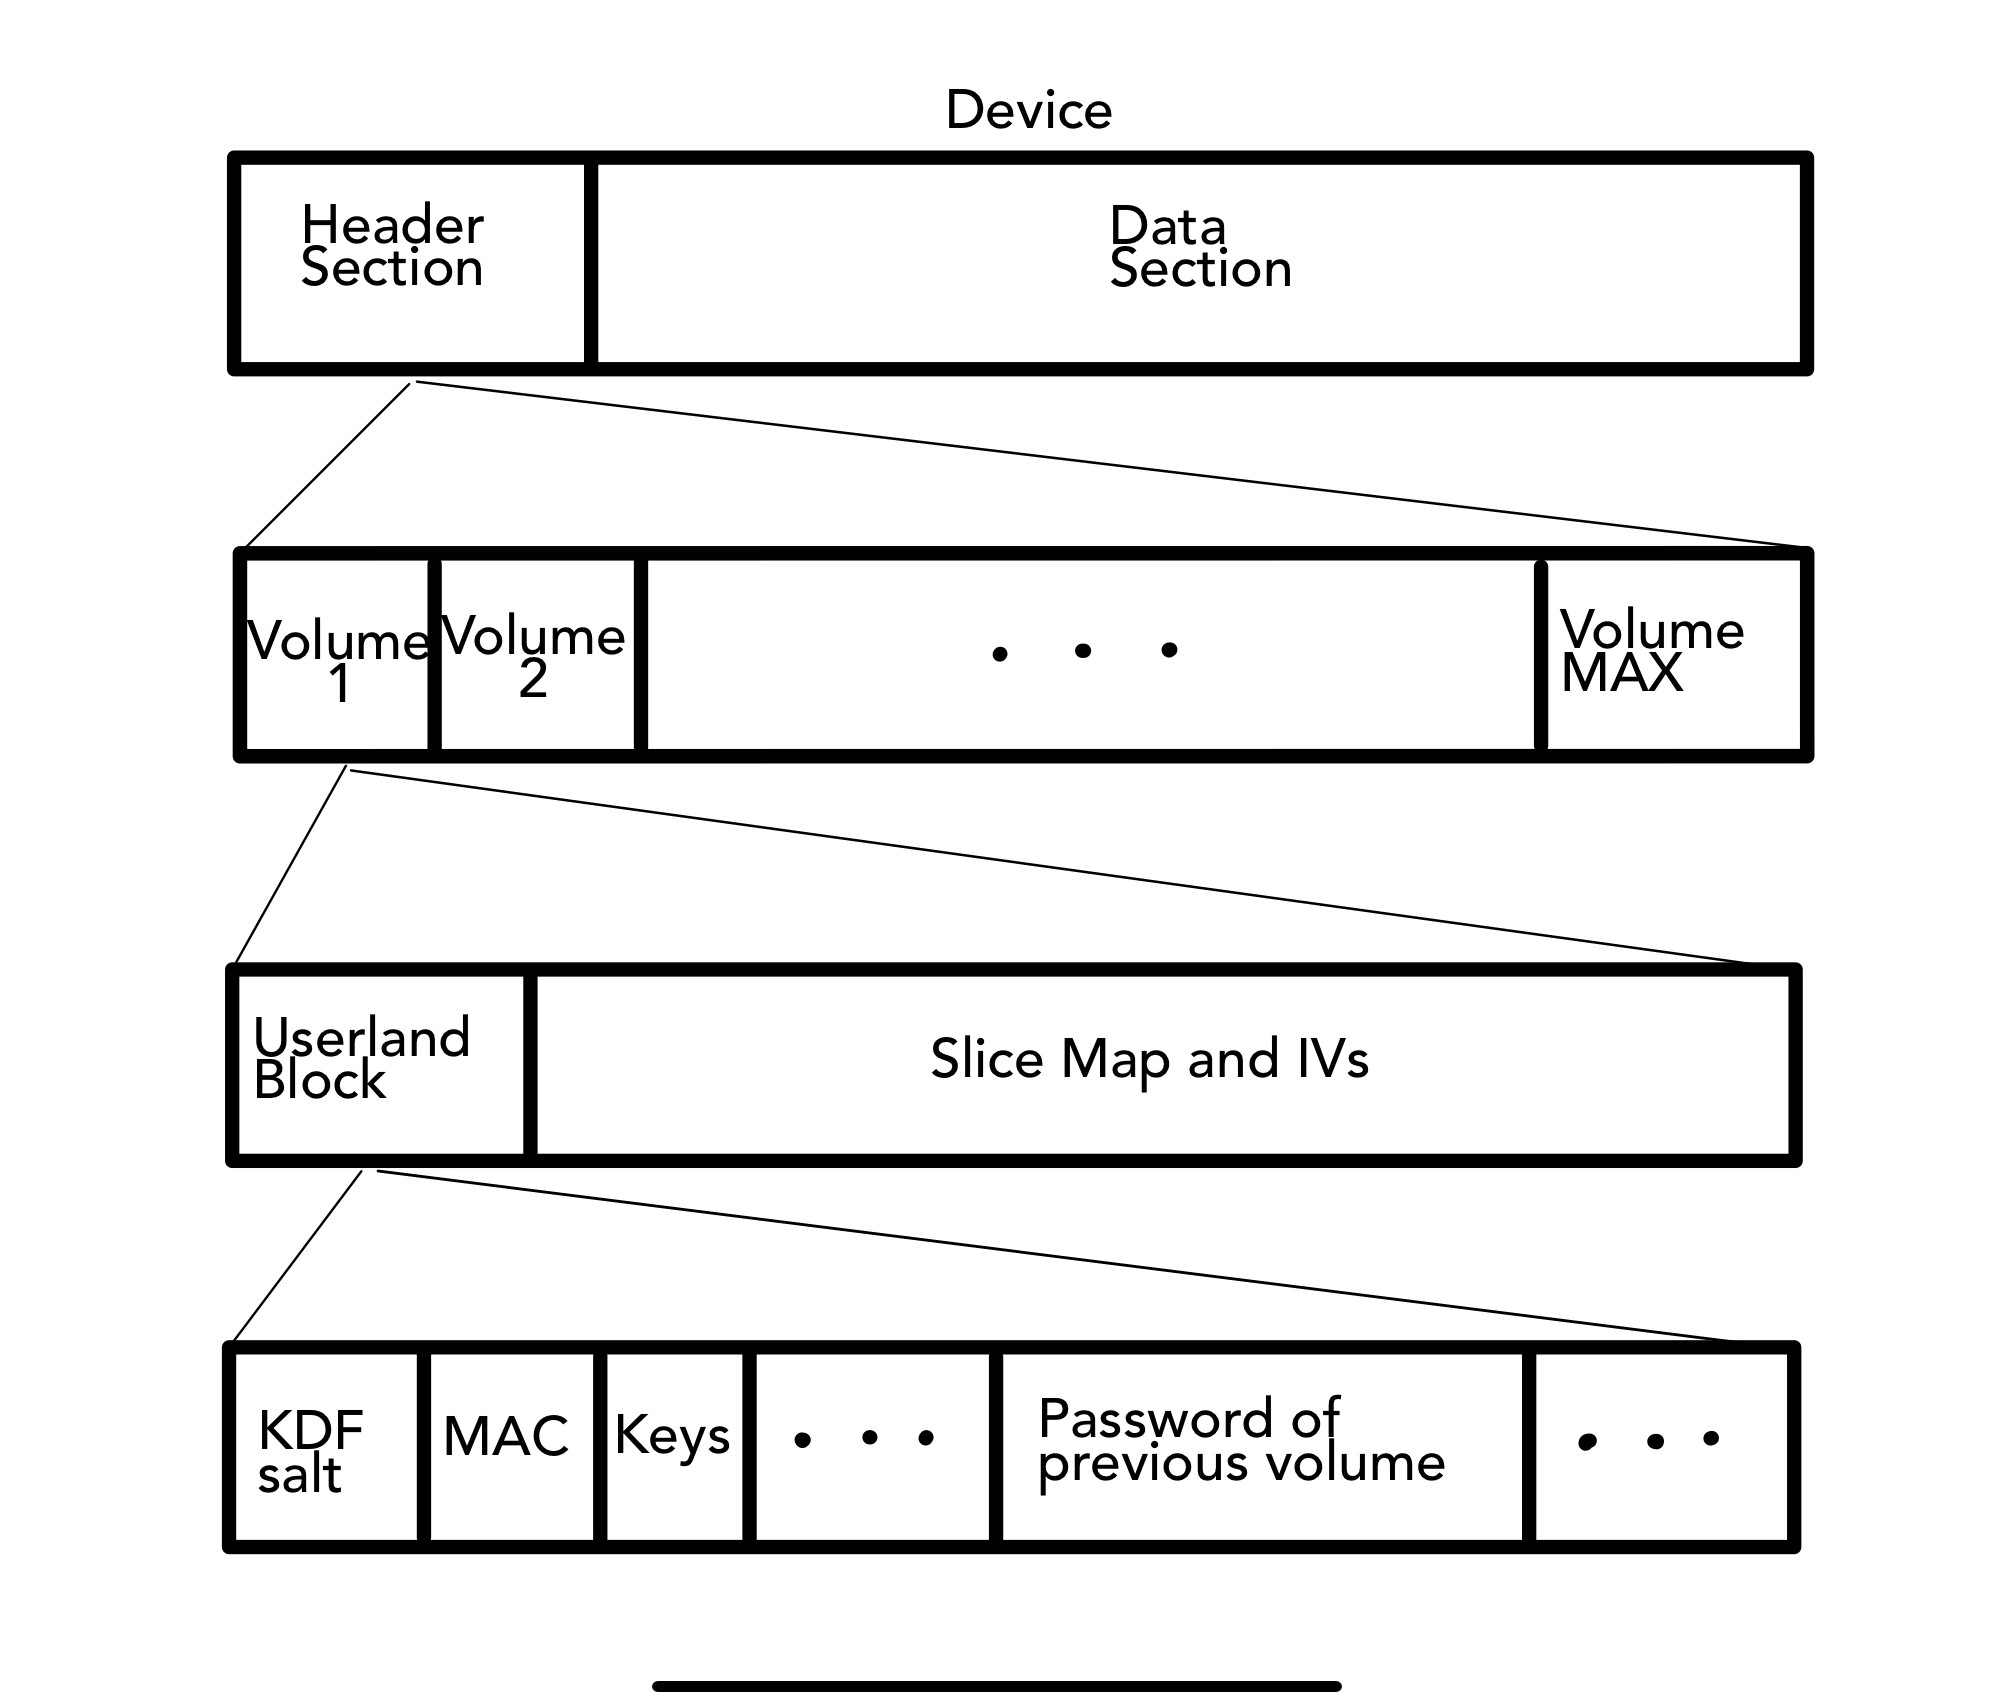
\includegraphics[width=0.8\textwidth]{Figures/sflc_layout.png}
\caption{Shufflecake disk layout}
\label{fig:sflc_layout}
\end{figure}

\section{Slice system}

When using Shufflecake, the storage space in the data section is divided into slices, which are groups of contiguous sectors. A physical space slice is made up of a number of data blocks, each preceded by a block containing all IVs (Initialization Vectors) used to encrypt those data blocks. When we see a slice from the logical space, the one that the user has access to, we only look at the data blocks. In this report, these slices will be referred to as physical and logical slices, respectively.

When a user manipulates data on a volume, they are operating so on logical slices. These are allocated as needed. A physical slice is assigned to each of these logical slices in order to effectively store the data on the underlying device storage. Because the assignments are uniformly random, consecutive slices in the logical space will end up interleaved in the physical space. Given that all volumes use the same data section with no boundaries between them, the slices of each volume will be interleaved with each others, as well as with the slices of all volumes. An example of this can be seen on figure \ref{fig:sflc_slices}.

\begin{figure}[ht]
\centering
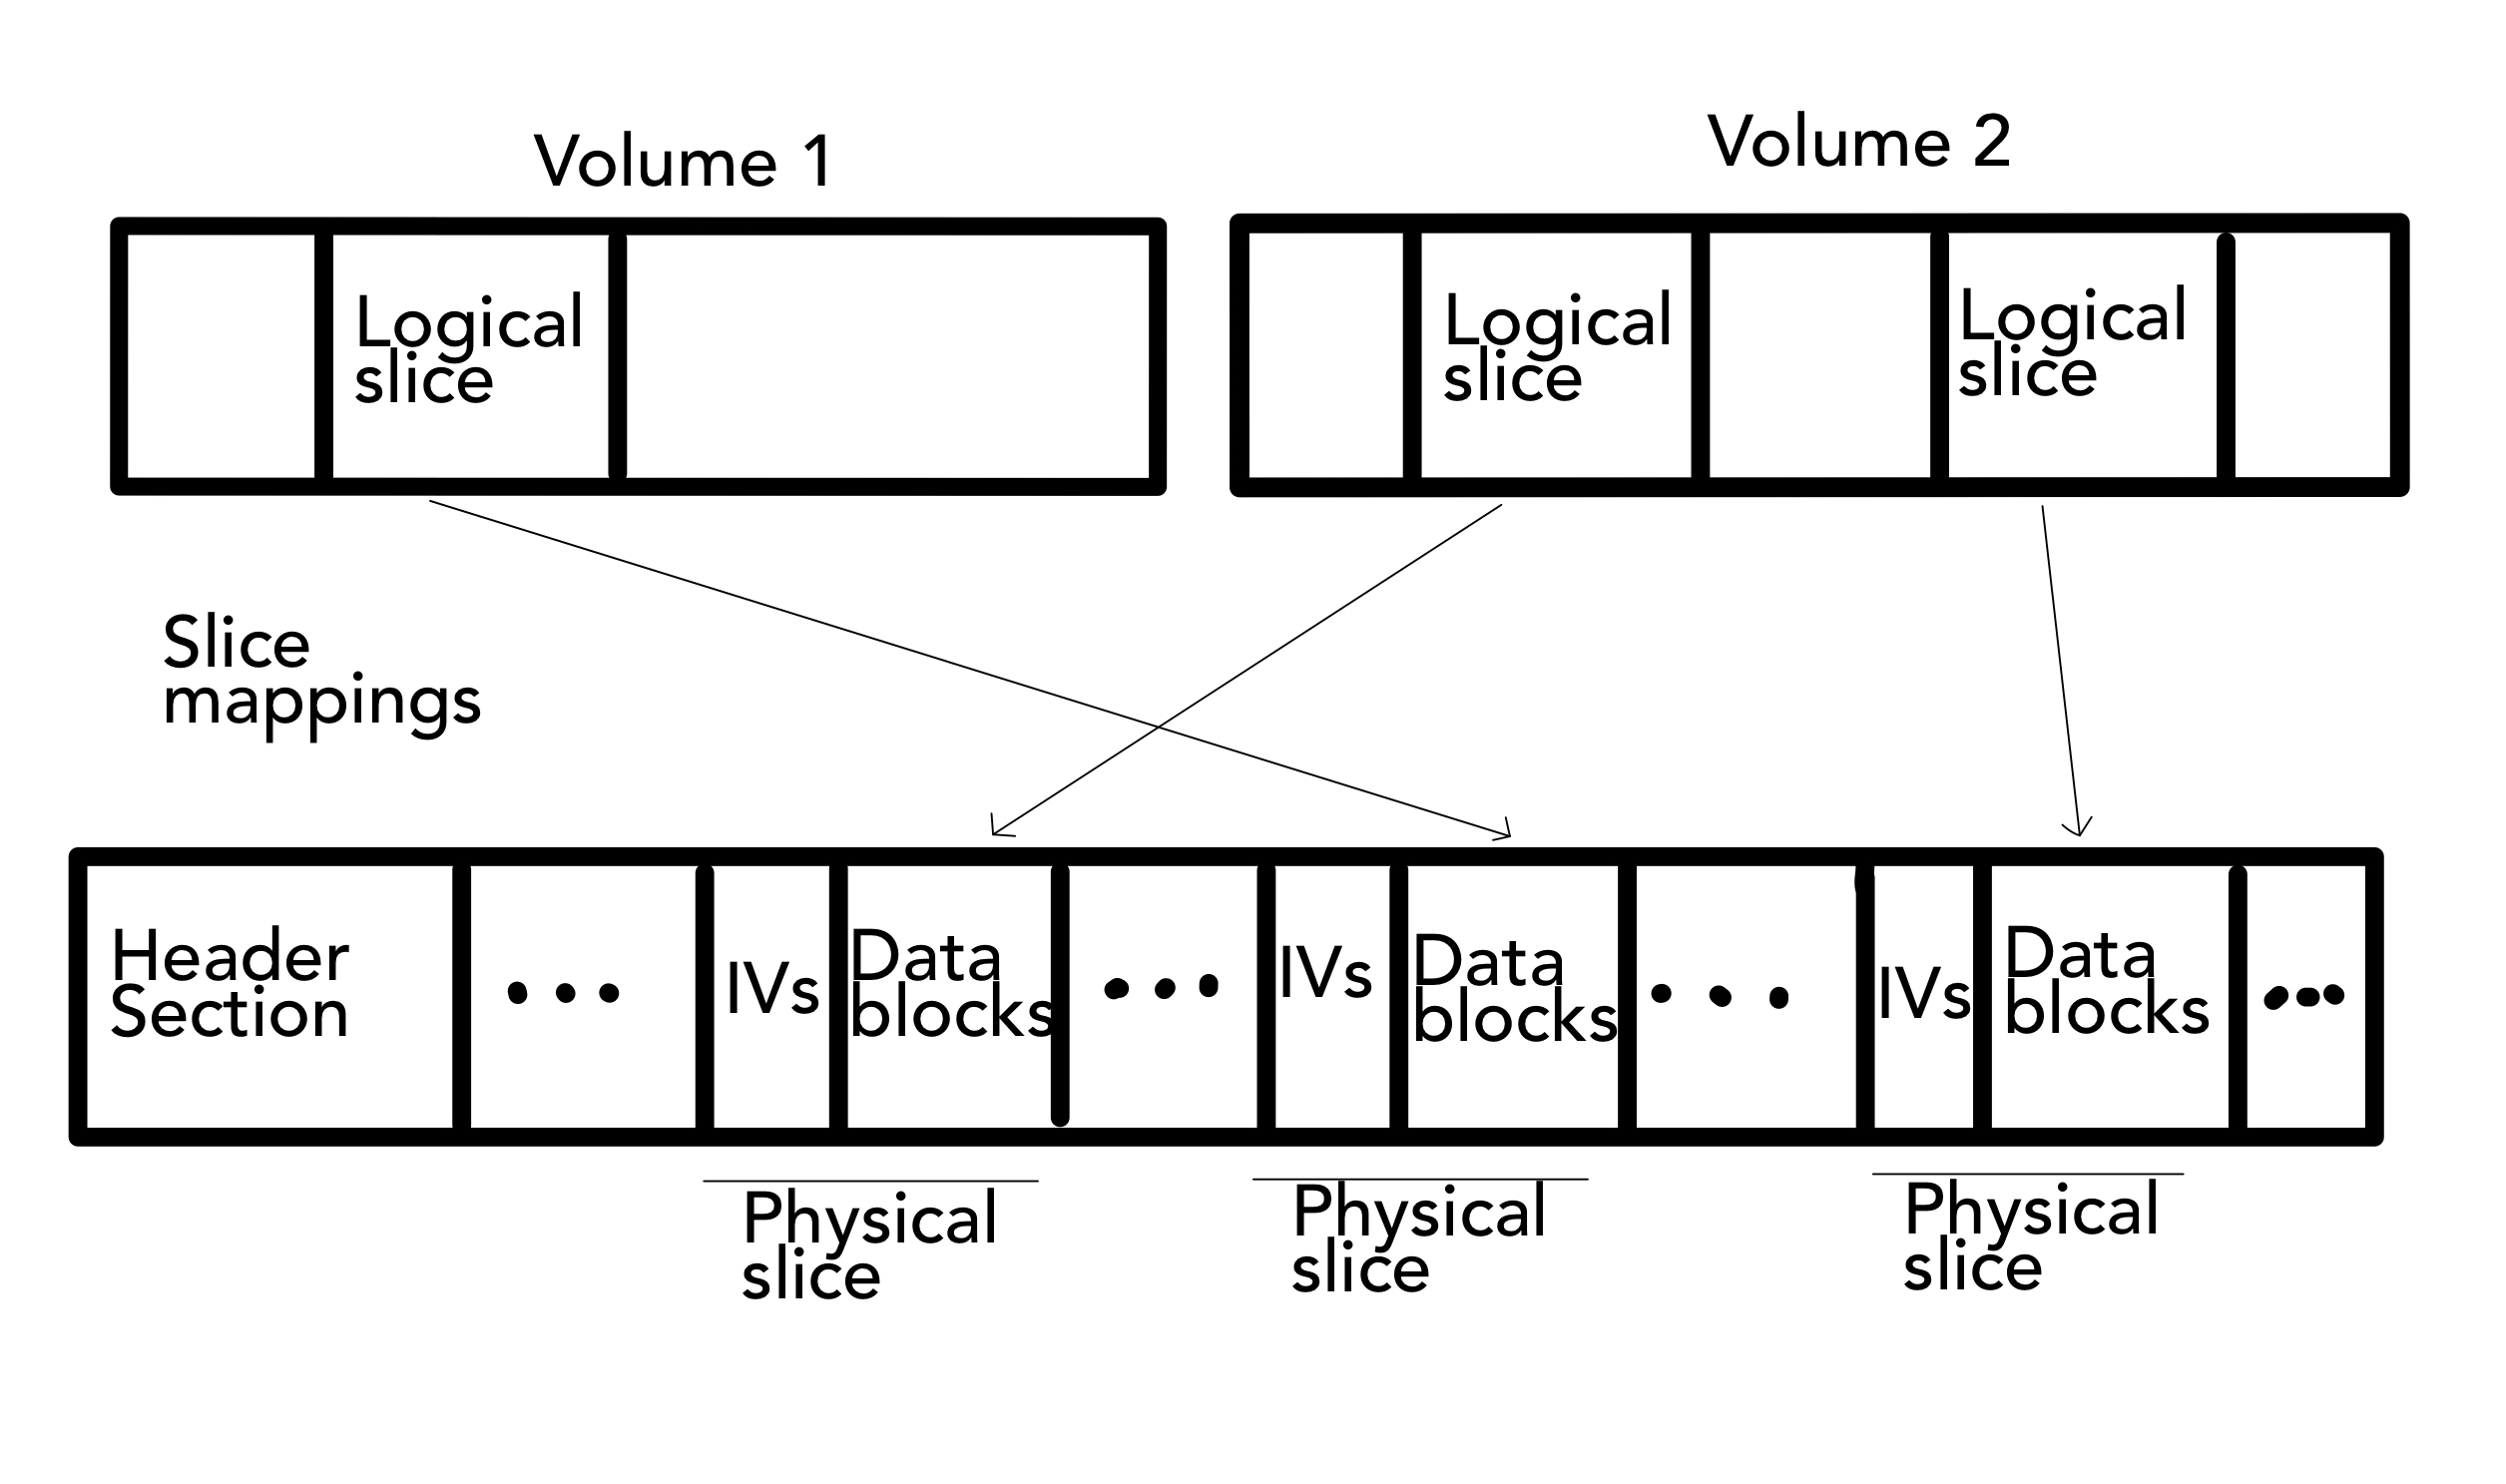
\includegraphics[width=0.8\textwidth]{Figures/sflc_slices.png}
\caption{Shufflecake slice system}
\label{fig:sflc_slices}
\end{figure}

Mappings are created for each volume to maintain the correspondence between the logical and physical slices. Those mappings are kept in RAM while the volumes are opened and persisted in the header section of the respective volume when it is closed so that they can be recovered the next time the volume is opened. The assignments are made lazily as needed, and each new physical slice is chosen from a list of free slices generated when the volumes are unlocked and kept entirely in RAM. This avoids conflicts when all volumes are used at the same time, but as we will see later, it may cause problems when some volumes are kept hidden while others are used.

The Shufflecake tool is only briefly discussed here, and the reader is directed to Elia Anzuoni's original paper "\textit{Hidden Filesystem Design and Improvement}"\cite{Anzuoni:297353} for more information.

\section{Drawbacks}

All volumes created using Shufflecake will appear to have the full capacity of the underlying storage device. This is a problem because it allows the user to overcommit resources and use more storage than is actually available, potentially corrupting existing data on those volumes. There are currently no safeguards in place, so it is the responsibility of the user to monitor and prevent this source of corruption.

Another potential issue is when some volumes are not unlocked while others are being used. Because of the plausible deniability aspect, the system has no way of distinguishing between hidden volume data and free space, and it may overwrite existing data when allocating new storage space. To mitigate this issue, volumes of lower secrecy are opened recursively. The user is not required to manually open them all. However, volumes of higher secrecy still may become corrupted.As a result, the recommended method of using Shufflecake is to always open all volumes when working on them. To reduce the risk of corruption when only some volumes are opened, usage should be limited to reads that have no effect on the underlying storage, but this is not always possible.

Finally, there is the possibility of an sThe original Shufflecake paper investigates some methods for extending security guarantees against multi-snapshot adversaries, such as the inclusion of "ghost filesystems." The goal of which is to make it appear as if there are always the maximum number of volumes used and to drown the signals of hidden volumes in noise. Shufflecake could support hidden operating systems stored on its hidden volumes to prevent information leakage caused by the OS. We'd like to see how redundancies can be implemented and how current mitigations perform under these new constraints.udden system crash, which could cause the storage device to behave in unpredictable ways. Crashes are especially a problem if they occur between the update of a data block and its corresponding IV block.

\let\clearpage\relax

%%%%%%%%%%%%%%%%
\chapter{Data corruption}
%%%%%%%%%%%%%%%%

In this project, we aim to make Shufflecake more resistant to the corruption which occurs when the storage device is used but not all volumes are unlocked by implementing some kind of redundancy. We also do it to make this solution more applicable in other contexts, such as decentralized or network storage, where this type of corruption is more likely to occur and must be addressed.

The first step is to identify and quantify how this corruption occurs in order to later determine whether the later proposed mitigations have the desired effect. Many factors can influence the level of corruption, the most evident of which are:
\begin{enumerate}
    \item The media type and physical capacity of the storage device
    \item The size and distribution of the slices
    \item The size and number of files stored on the hidden volumes
    \item The number of concealed volumes
    \item The operations carried out on the volumes
\end{enumerate}

\section{Testing framework}

To test a credible usage scenario, a USB key with a fixed size of 1GB was used as the storage device. For the time being, the slice size in Shufflecake is fixed at 1MB and is allocated as needed; there is no preallocation or batch allocation that could influence results; however, to ensure that they are used consistently, the test files used will be 1MB or multiples of 1MB. The testing will begin with two Shufflecake volumes, one serving as the hidden volume and the other as the decoy. The number of volumes will be increased later in the testing process if needed. Finally, Shufflecake was created for Linux headers 5.15, and the driver is heavily reliant on them, so all tests will be performed with this version. It should also be noted that Shufflecake provides the option to fill the storage device with random bytes before creating the volumes; while this can be very useful in real-world use cases, it was skipped in testing because it had no effect on the results here.

The general testing framework will look something like this:
\begin{enumerate}
    \item The volumes are created and opened
    \item Some test files are written on the hidden volume
    \item All volumes are closed
    \item Only the decoy volume is opened and some dummy files are written on it
    \item The hidden volume is opened and the test files are verified
\end{enumerate}
Steps 3 and 4 are repeated several times in a row to observe the evolution of the corruption. In the corruption analysis section of this project, each iteration will be referred to as a corruption round.

\section{Implementation specifics}

To be used to store files and run our tests, the Shufflecake volumes must be formatted with some filesystem. Ext4\cite{ext4} was chosen because it is currently the most widely used file system on Linux distributions. This is good for plausible deniability because it does not raise suspicion. It also works really well with the slice system, by filling the slices up as much as possible before requesting new ones, which limits the internal fragmentation of slices and so the space utilization. Additionally, it works really well with the slice system because it maximizes the utilization of existing slices before asking for new ones, which reduces internal slice fragmentation\cite{Anzuoni:297353}. The presence of a filesystem, however, adds an additional constraint. As the hidden volume space becomes corrupted, the filesystem may become corrupted and cease to function, preventing any further testing. As a result, the filesystem is checked using the Linux utility fsck just before the test files are checked.

The test and dummy files are made up of random bytefiles generated by the kernel random number generator. In this case, /dev/urandom was chosen over /dev/random because it is faster and true randomness is not required in those tests. Bytefiles were chosen over specific file formats to prevent codecs reading those file formats from correcting some corruption, influencing the results.

To simulate light, moderate, and heavy workloads, three types of tests were produced using dummy files of small (20 * 1MB per round), medium (20 * 2MB per round), and large sizes (20 * 4MB per round) for a set number of rounds. Those numbers were chosen so that the total space used remains less than the storage device true physical capacity, preventing corruption due to overcommitment of storage space. The tests were also repeated several times to obtain an average of the rate of file corruption.

\section{Checksum analysis}

There are many ways of examining test files that have been corrupted. To begin, the checksums of the files were used to provide a global overview of the file corruption in the hidden volume. In this first test, 100 * 1MB test files were created in the hidden volume, and their checksums were saved and compared after each round of corruption. Each round, twenty dummy files are added to the decoy volume while the hidden volume is not opened, potentially corrupting parts of it.

\begin{figure}[ht]
     \centering
     \begin{subfigure}[b]{0.3\textwidth}
         \centering
         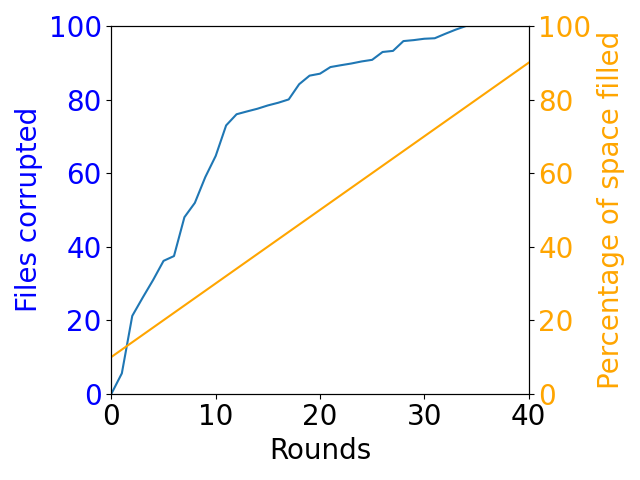
\includegraphics[width=\textwidth]{Figures/average_checksum_corrupt_1MB.png}
         \caption{Light workload}
         \label{fig:checksum_light}
     \end{subfigure}
     \hfill
     \begin{subfigure}[b]{0.3\textwidth}
         \centering
         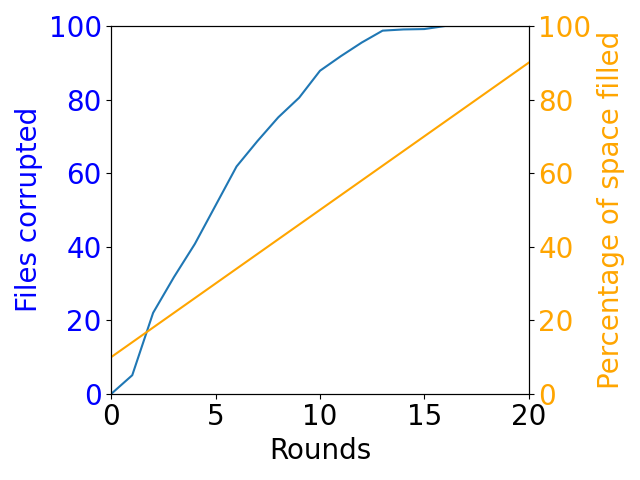
\includegraphics[width=\textwidth]{Figures/average_checksum_corrupt_2MB.png}
         \caption{Medium workload}
         \label{fig:checksum_medium}
     \end{subfigure}
     \hfill
     \begin{subfigure}[b]{0.3\textwidth}
         \centering
         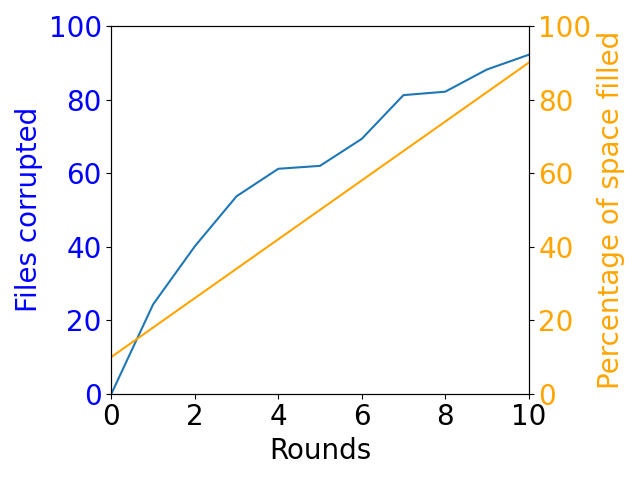
\includegraphics[width=\textwidth]{Figures/average_checksum_corrupt_4MB.png}
         \caption{Heavy workload}
         \label{fig:checksum_heavy}
     \end{subfigure}
        \caption{Checksum corruption analysis}
        \label{fig:checksum_analysis}
\end{figure}

The blue line in figures \ref{fig:checksum_light}, \ref{fig:checksum_medium} and  \ref{fig:checksum_heavy} represents the number of corrupted test files in small, medium and light workloads respectively. The corruption is detected by a change in the file checksum. Another orange line was added to show the amount of storage space used on the device. The results of this first test are not very telling; a large number of files become corrupted very quickly, and there is no way of knowing how corrupted they become. The size of the dummy files does not appear to make a significant difference.

It should be noted that in most cases, the corruption was not detected by a change in checksum, but rather by files going missing during testing because of filesystem events. During the filesystem check that occurs before the test files are verified, I observed three types of events that occurred on a regular basis (almost in every test instance). The first occurred when the filesystem journal became corrupted. In this case, fsck repaired the filesystem successfully every time, with no noticeable effect on the test files. The other two events occurred when the superblock or the directory structure became corrupted, and in both cases, a large number of files went missing shortly afterwards. Those files are probably unlisted during the filesystem reconstruction, and even if they are still on the disk, they are no longer registered by the filesystem. 

\section{Byte-level analysis}

To continue on the analysis, the corruption is now monitored on a byte level. Instead of saving the checksums of the test files, a local copy is directly saved on another volume for this test. After each round, the hidden files are compared byte by byte to their reference copy to see if there are any differences. Aside from that, the same testing methodology as before is used.

\begin{figure}[ht]
     \centering
     \begin{subfigure}[b]{0.3\textwidth}
         \centering
         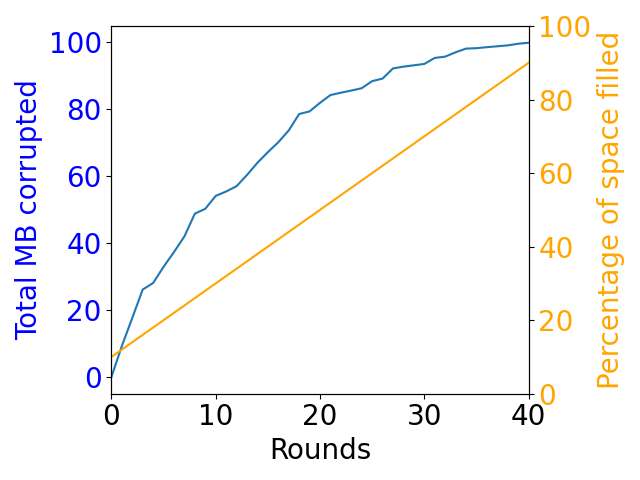
\includegraphics[width=\textwidth]{Figures/sum_byte_corrupt_1MB.png}
         \caption{Light workload}
         \label{fig:byte_light}
     \end{subfigure}
     \hfill
     \begin{subfigure}[b]{0.3\textwidth}
         \centering
         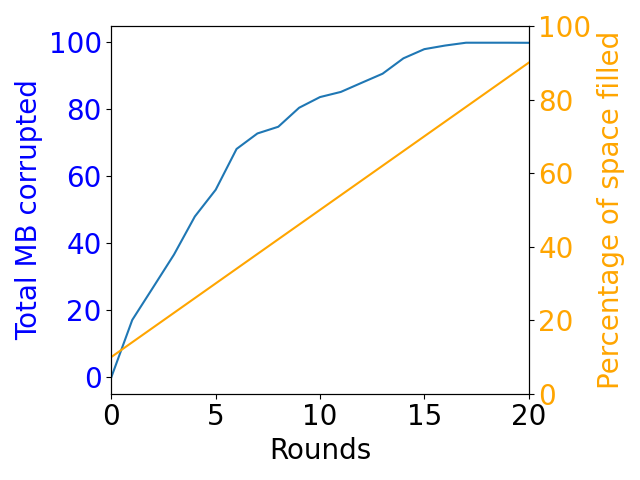
\includegraphics[width=\textwidth]{Figures/sum_byte_corrupt_2MB.png}
         \caption{Medium workload}
         \label{fig:byte_medium}
     \end{subfigure}
     \hfill
     \begin{subfigure}[b]{0.3\textwidth}
         \centering
         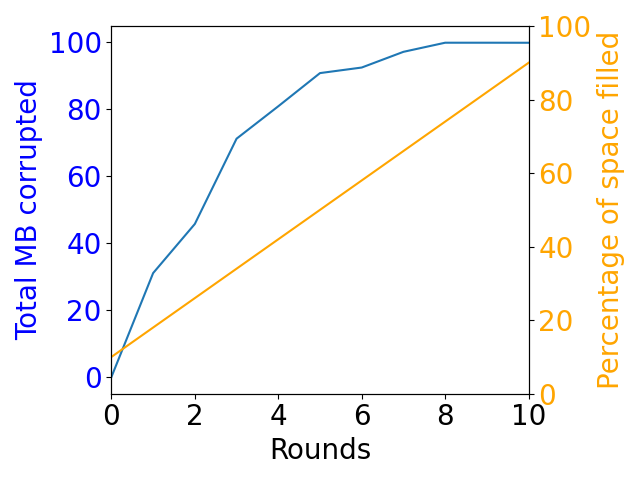
\includegraphics[width=\textwidth]{Figures/sum_byte_corrupt_4MB.png}
         \caption{Heavy workload}
         \label{fig:byte_heavy}
     \end{subfigure}
        \caption{Byte-level corruption analysis}
        \label{fig:byte_analysis}
\end{figure}

The blue line in figures \ref{fig:byte_light}, \ref{fig:byte_medium} and \ref{fig:byte_heavy} now represents the amount of megabytes corrupted for all test files. The outcomes are very similar to the previous ones. Because we consider the bytes individually rather than all together (using the checksum), the rate of corruption appears to be slightly slower.

Again during testing, filesystem errors appear to be the primary vector of corruption, consuming entire files at once and making it difficult to extract useful information from the results. We can showcase this phenomenon on specific test files.

\begin{figure}[ht]
     \centering
     \begin{subfigure}[b]{0.45\textwidth}
         \centering
         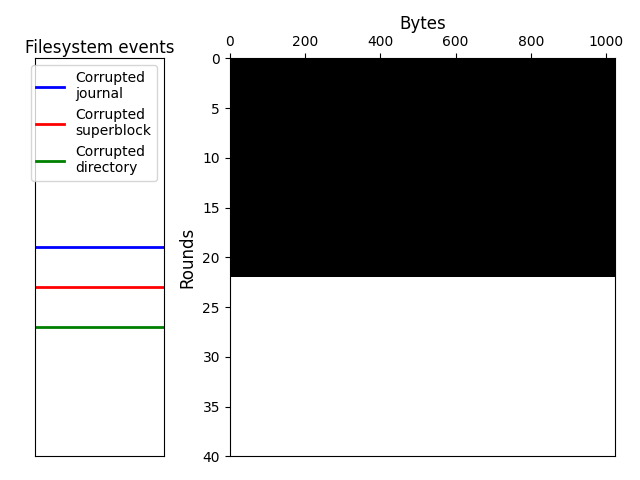
\includegraphics[width=\textwidth]{Figures/visual_file_corruption1.png}
         \caption{First example file}
         \label{fig:byte_file1}
     \end{subfigure}
     \hfill
     \begin{subfigure}[b]{0.45\textwidth}
         \centering
         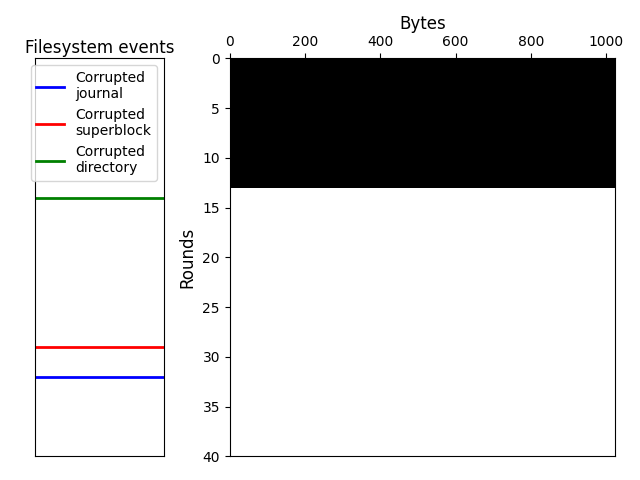
\includegraphics[width=\textwidth]{Figures/visual_file_corruption2.png}
         \caption{Second example file}
         \label{fig:byte_file2}
     \end{subfigure}
        \caption{Byte-level corruption visualization}
        \label{fig:byte_visual}
\end{figure}

On figures \ref{fig:byte_file1} and \ref{fig:byte_file2}, a single test file is monitored. Its bytes are shown in black and change to white when they become corrupted. We can see on the left when filesystem events happen and that they drive the corruption. Additional tests were performed to examine the frequency of filesystem events and see if they followed any pattern, but no conclusive results were found, so the results will not be included here. As previously stated, it is possible that the majority of the missing files are still present on disk but are no longer listed by the filesystem.

It is also possible that some of these files are still registered by the filesystem, but not in the same way they were before. When repairing the filesystem, the fsck utility will attempt to recover corrupted file fragments and place them in the volume lost+found directory. Those files could be recovered and even rebuilt directly from disk, but this task appears to be beyond the scope of this project. Furthermore, such modifications would be highly filesystem-dependent, which contradicts the Shufflecake tool philosophy and the plausible deniability aspect in general.

\section{Slice-level analysis}

Instead of staying on the byte-level and dealing with all the aforementioned filesystem issues, the focus is shifted to the slices that Shufflecake employs as storage units. When a slice is reused by an unlocked volume while it is still in use by a locked volume, it is considered corrupted. When we base the analysis on slices, the results become much clearer visually like we can see in figure \ref{fig:slice_visual}.

\begin{figure}[ht]
\centering
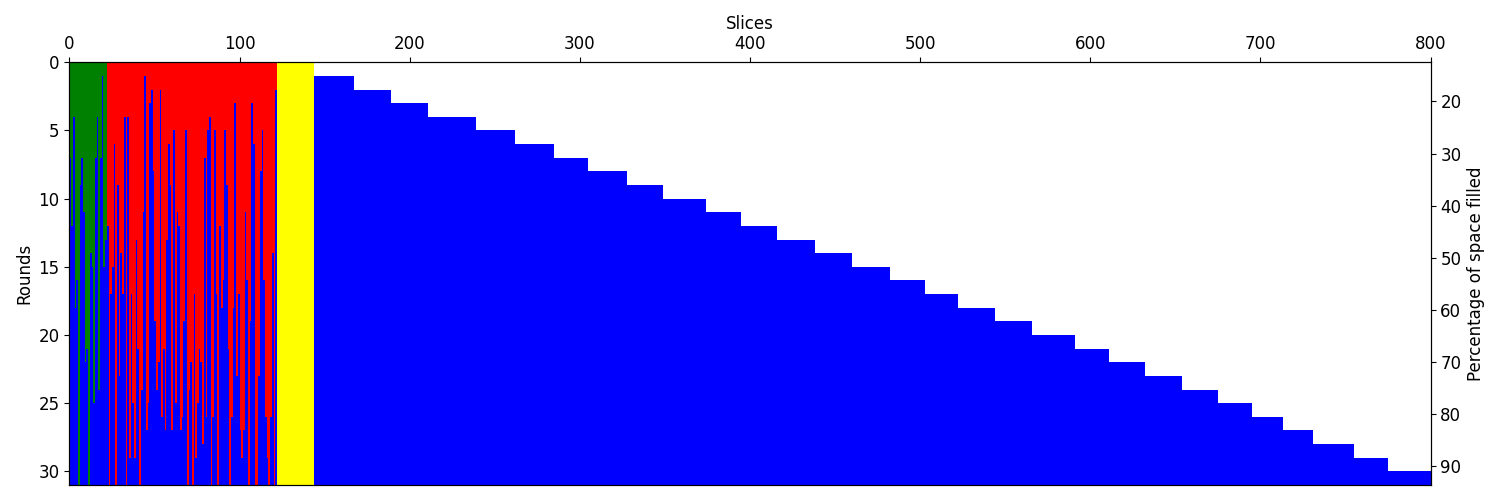
\includegraphics[width=\textwidth]{Figures/visual_slice_corruption.png}
\caption{Slice corruption visualization}
\label{fig:slice_visual}
\end{figure}

The slices on figure \ref{fig:slice_visual} are colored when they are assigned to a specific Shufflecake volume space. The slices assigned to the hidden volume, in green and red, are for the filesystem data and test files, respectively. The same thing is done in yellow and blue for the decoy volume, this time with the dummy files instead of the test files. It should be noted that the slices are not necessarily contiguous in memory, but they are shown as such here for clarity. The test settings were also tweaked slightly because the previous ones allowed for some corruption due to overcommitment of the space in some cases. New settings were chosen for light (25 * 300KB per round), medium (25 * 1MB per round) and heavy (25 * 3MB per round) workloads.

We can see that as the corruption rounds progress, the Shufflecake software allocates more and more slices to the decoy volume. It will also occasionally allocate slices that were previously allocated to the hidden volume (which is hidden at this point, so there is no way to check if those slices are already in use), corrupting them. Because the decoy volume is always unlocked, its slices are never corrupted, and they can be removed from the figure to focus on the hidden volume.

\begin{figure}[ht]
\centering
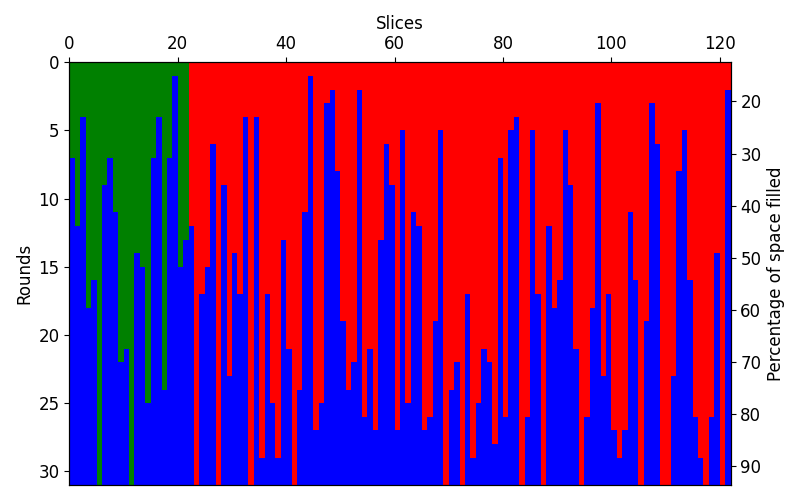
\includegraphics[width=0.7\textwidth]{Figures/visual_slice_corruption_shorted.png}
\caption{Slice corruption visualization; only hidden volume}
\label{fig:slice_visual_shorted}
\end{figure}

The corruption can be seen in figure \ref{fig:slice_visual_shorted} as the test progresses. Slices allocated to test files (in red) are reallocated to dummy files, and the data is overwritten; slices allocated to filesystem data (in green) are reallocated to dummy files, resulting in long-term filesystem consistency errors. However, unlike in the past, the filesystem events do not impede the rest of the test because we are not testing the files themselves.

When a slice becomes corrupted, its original content is overwritten by the content of the decoy slice. Even though the slice technically now belongs to both volumes according to the slice map, it can only hold the data that was last written to it. The hidden volume still believes the slice contains its data, but attempting to read it yields gibberish. If the overwritten slice contained filesystem data, this could result in those filesystem consistency errors. It may also attempt to write data back onto it, and both volumes will compete for ownership of the slice. This is likely to occur if we attempt to repair the filesystem of the corrupted volume without first resolving the slice mappings duplicates. Any mitigation implemented to add redundancy should be applied to all volume slices, whether they are filesystem slices or data slices.

In this configuration, a slice cannot get corrupted multiple times in a row. As soon as its gets corrupted, it also belongs to the decoy volume which will prevent it from being corrupted again. This logic can be extended to a situation with multiple hidden volumes. If we are forced to surrender some of our volumes under coercion, the volumes will be handed over in the order of their secrecy. It makes no sense to try to conceal a volume once it has been discovered. Even if the volumes are opened and closed multiple times in different configurations, if we follow the reasonable assumption that the exposed set of volumes is only going to expand, we can be confident that the physical slices will not be corrupted more than once in a row.

\section{Rate of corruption}

We can now confirm that the slice corruption rate is fully probabilistic. This makes sense given that the newly allocated slices are chosen at random from among the available ones. When we only have access to the decoy volume, the probability of selecting a slice from the hidden volume is:

\[ \frac{Hidden\ volume\ slices\ -\ Corrupted\ slices}{Total\ slices\ -\ Decoy\ volume\ slices} \]

We can compare the corruption rate of the hidden volume slices in a specific scenario and compare it to the prediction made by our formula.

\begin{figure}[ht]
     \centering
     \begin{subfigure}[b]{0.3\textwidth}
         \centering
         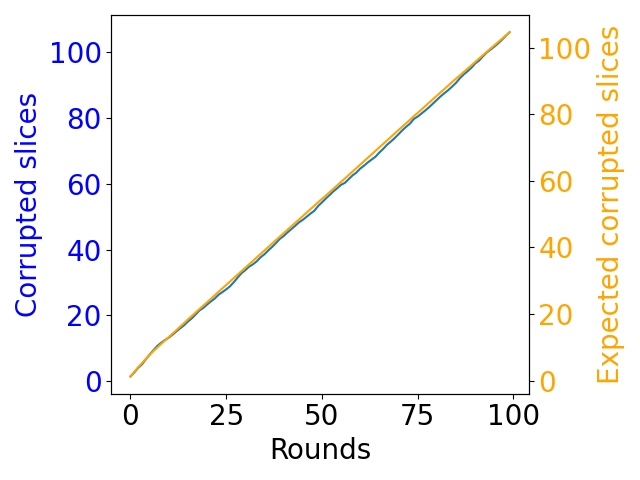
\includegraphics[width=\textwidth]{Figures/corruption_rate300KB.png}
         \caption{Light workload}
         \label{fig:slice_light}
     \end{subfigure}
     \hfill
     \begin{subfigure}[b]{0.3\textwidth}
         \centering
         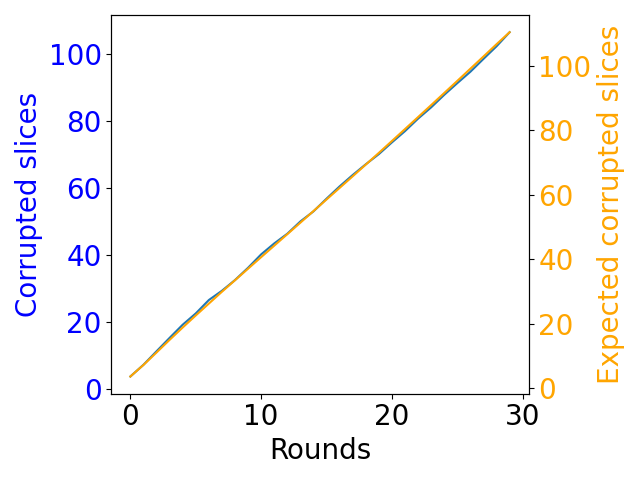
\includegraphics[width=\textwidth]{Figures/corruption_rate1MB.png}
         \caption{Medium workload}
         \label{fig:slice_medium}
     \end{subfigure}
     \hfill
     \begin{subfigure}[b]{0.3\textwidth}
         \centering
         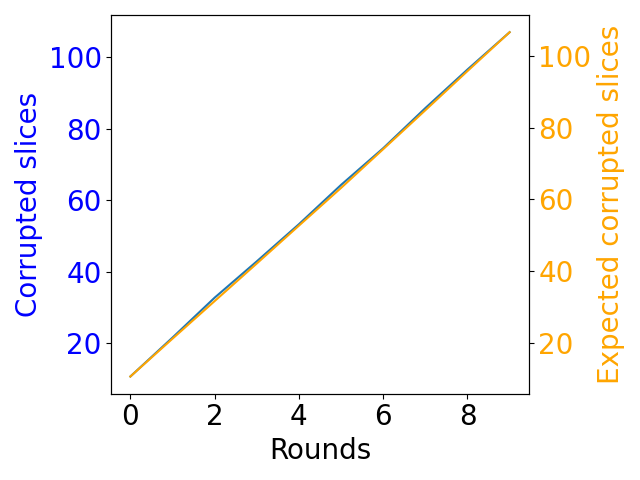
\includegraphics[width=\textwidth]{Figures/corruption_rate3MB.png}
         \caption{Heavy workload}
         \label{fig:slice_heavy}
     \end{subfigure}
        \caption{Slice corruption analysis}
        \label{fig:slice_analysis}
\end{figure}

The results, observable in figures \ref{fig:slice_light}, \ref{fig:slice_medium} and \ref{fig:slice_heavy}, are consistent across all workloads and file sizes tested. An interesting aspect is that the corruption rate of the slices remains relatively constant over time. This was unexpected because the ratio of hidden slices to available remaining slices is expected to increase as we fill up the storage over the rounds. We expect to corrupt more and more slices each round. However, because hidden slices can only be corrupted once, as more and more are corrupted, the number of available slices decreases. Both trends cancel each other out, and the slice corruption remains nearly constant.

In Shufflecake, the slice size is set to 1MB. With this information, we could easily convert our formula to work in terms of bytes. In this conversion, we have to keep in mind that the available storage is frequently different from the device advertised storage. It should also be noted that both Shufflecake and the filesystem installed on each volume have a storage overhead to take into account.

Because all slices are chosen independently of one another, slice allocations are also independent of one another. For large files, this means that the probabilities can be added up at each step for each new slice allocated. It also implies that there should be no difference if we repeat this experiment with multiple hidden volumes.

\let\clearpage\relax

%%%%%%%%%%%%%%%%%%%%%%%%
\chapter{Mitigations}
%%%%%%%%%%%%%%%%%%%%%%%%

We intend to use redundancy mitigations to reduce this corruption rate. We cannot prevent this corruption while maintaining Shufflecake plausible deniability guarantees, so we will instead focus on attempting to repair the corruption after it has occurred.

To make this repair possible, we will replicate the content of the slices, effectively maintaining a 1-to-1 copy of the slices at all times. This is the replication part.

Then comes the repair part, in which we inspect the slices for corruption each time the volumes are opened. We do this by looking for inconsistencies in the slice maps, which occur when different volumes assign the same physical slices to different logical slices, like we can see in figure \ref{fig:sflc_disambiguate}. At this point, we want to disambiguate the situation by assigning a new physical slice to one of the volumes and leaving the other, but which volume gets to keep the original physical slice?

\begin{figure}[ht]
\centering
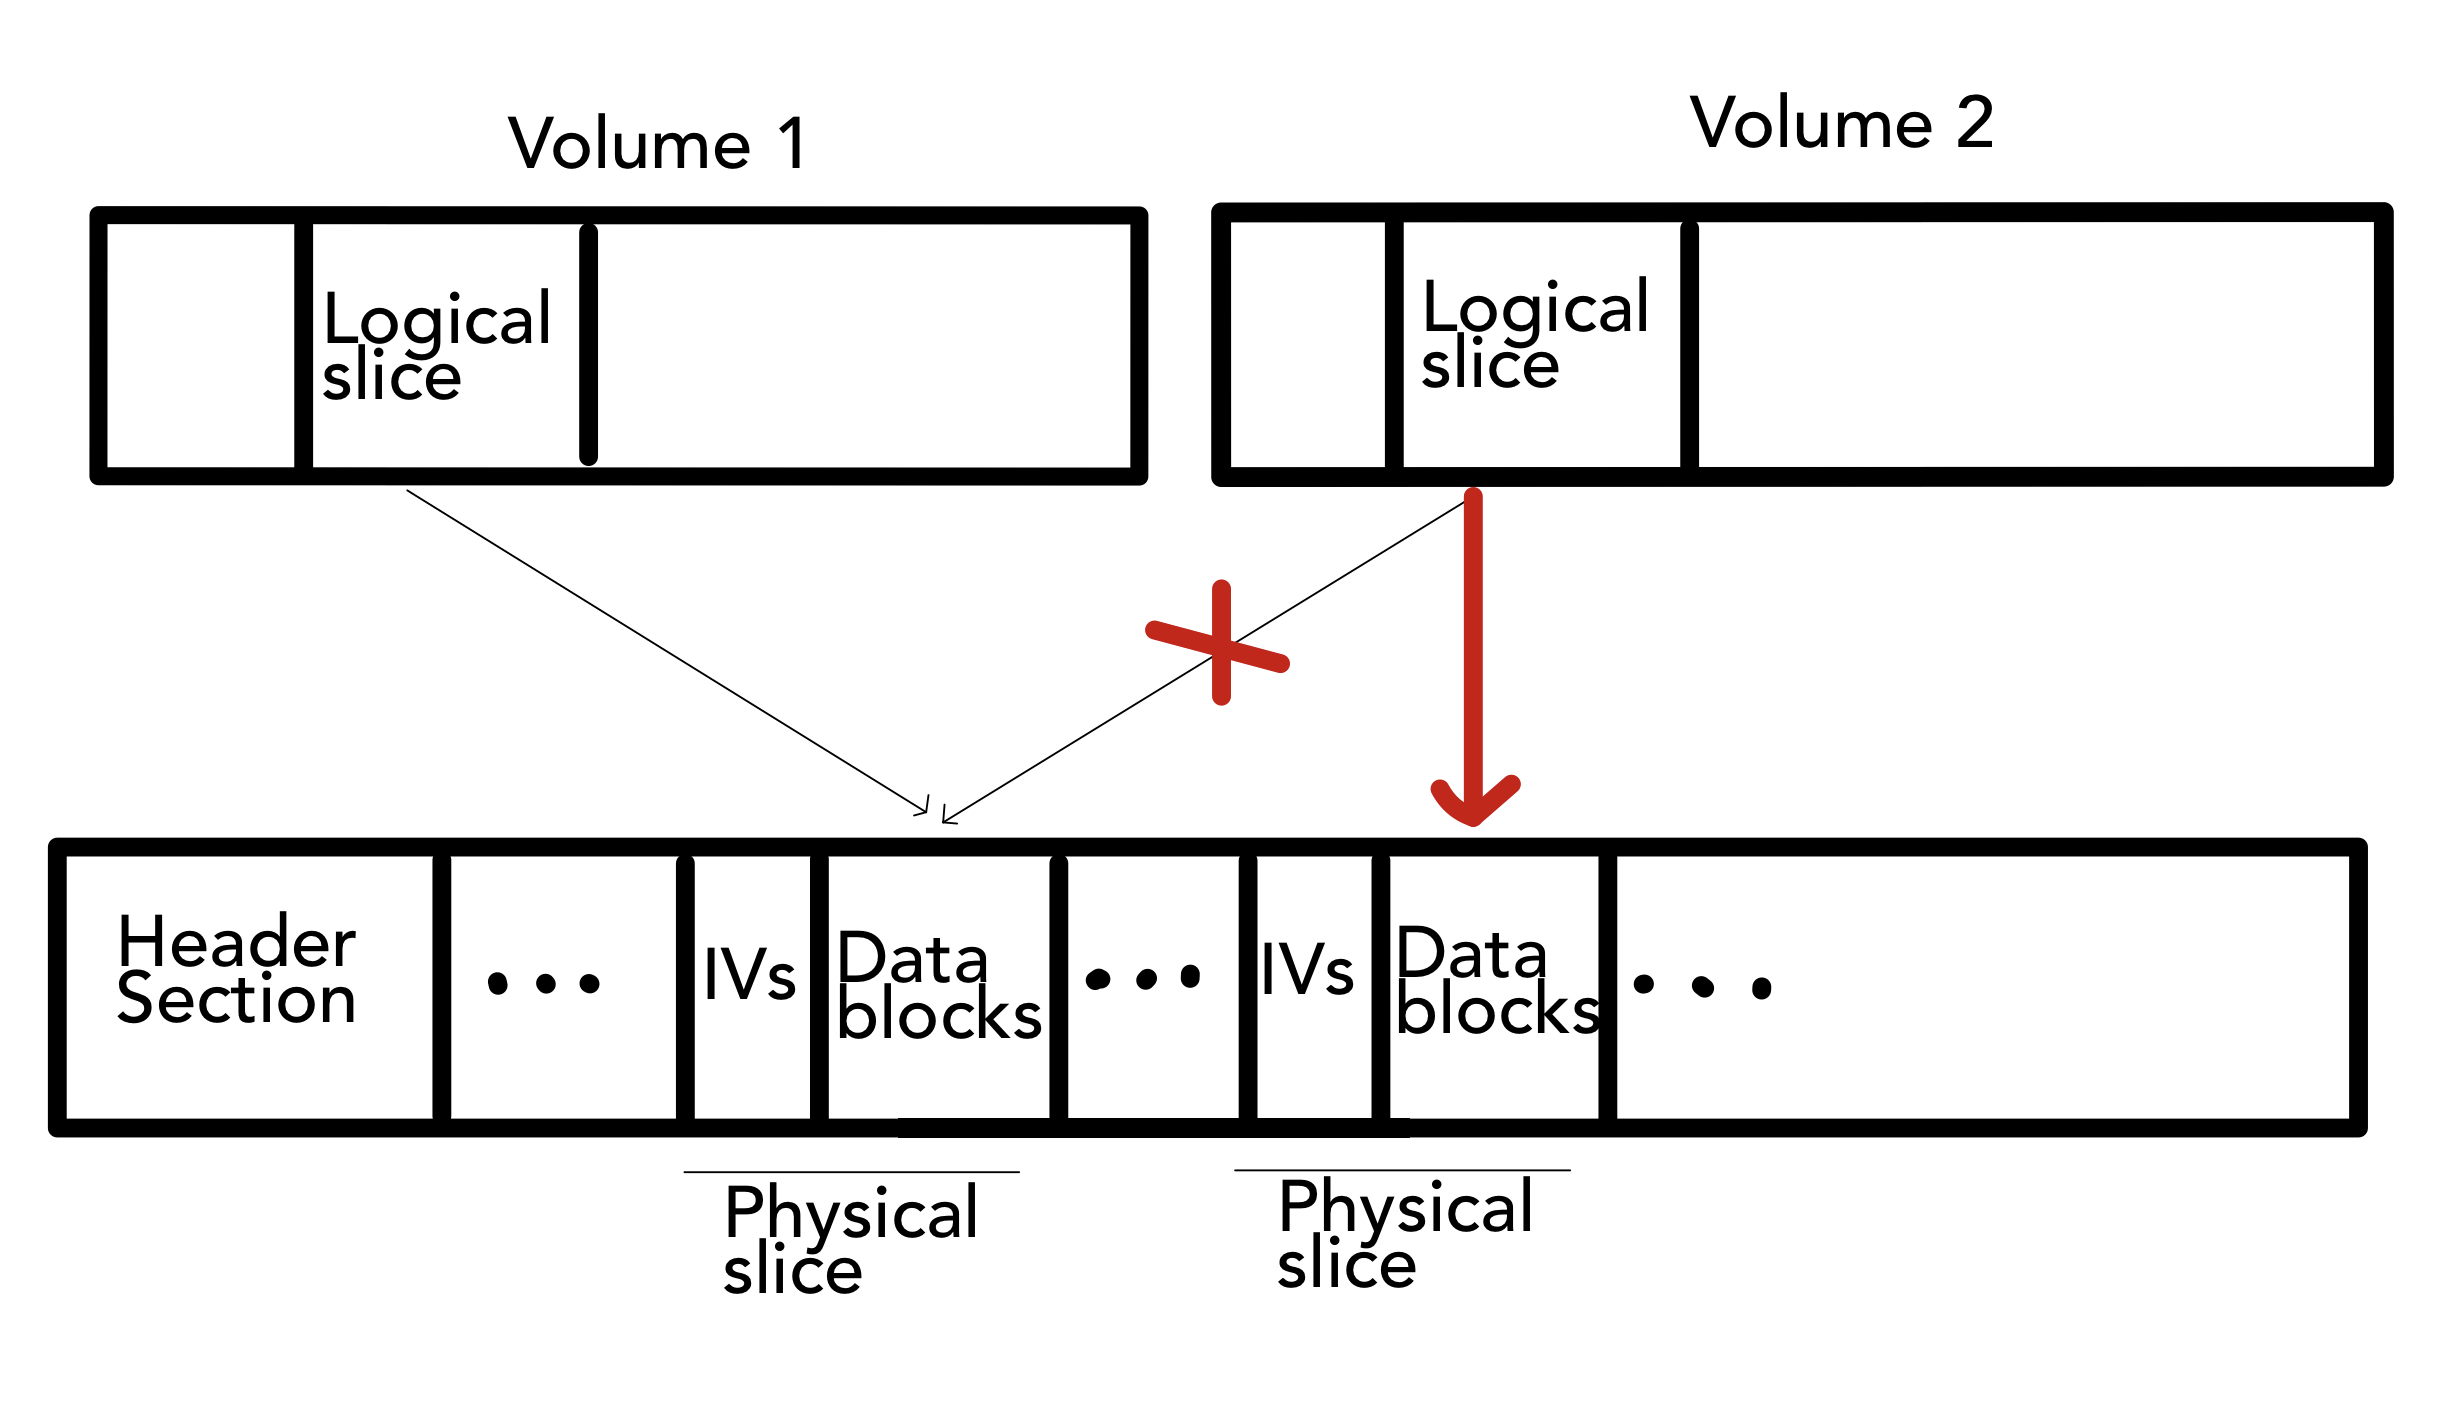
\includegraphics[width=0.8\textwidth]{Figures/slice_disambiguate.png}
\caption{Slice disambiguation process}
\label{fig:sflc_disambiguate}
\end{figure}

We ultimately decided to leave the slice to the volume with the least amount of secrecy. This may appear to be counter-intuitive, as the more secret the data, the more valuable it should be, but this paradigm is reversed when dealing with plausible deniability. Because the less secret files will mostly be used as decoys, it is critical that they remain as untouched as possible. The files used as a decoy must appear as common and unremarkable as possible, and moving them around only increase the risk of further corrupting them.

Furthermore, if multiple physical slices are assigned to the same volume, its content will be overwritten by the last volume to which the slice was allocated. Because of the hierarchy of secrecy that Shufflecake operates on, this last volume will always have the lowest secrecy of the two. When a volume is opened, all volumes with lower secrecy than its own are automatically and recursively opened. The driver can only reallocate a slice that already belongs to another volume if it has no knowledge of that volume, which means it has not been opened and is not of an higher secrecy.

In short, we keep the volume that "corrupted" the slice by making it its own, and we allocate a new slice to the other one, which we will attempt to fill with its original content using the backup slice.

One important point to note is that we do not need to implement this redundancy on the volume with the highest level of secrecy because, regardless of how we use Shufflecake, this volume will always be open and thus cannot be corrupted by other volumes. It represents the bare minimum of secrecy that we can work with, and it serves as the primary decoy. 

\section{MDADM approach}

First, we will try to use existing software solutions because they are the easiest to implement. The design implementation we are attempting is very similar to a RAID partition, in this case mirroring, so RAID1. Hence, we will try to use a RAID software manager. This may allow also us to easily expand the redundancy to other RAID schemes such as RAID5 or RAID6 for a better balance of data safety and storage utilization.

Mdadm is a Linux tool for managing and monitoring RAID partitions\cite{mdadm_man}. It operates on block devices like the device mapper framework used in Shufflecake. This makes it very simple to use in our situation. We can create and open the Shufflecake volumes and then use their block devices corresponding with mdadm to create additional block devices that will serve as our RAID array. An overview can be seen in figure \ref{fig:red_mdadm}.

\begin{figure}[ht]
\centering
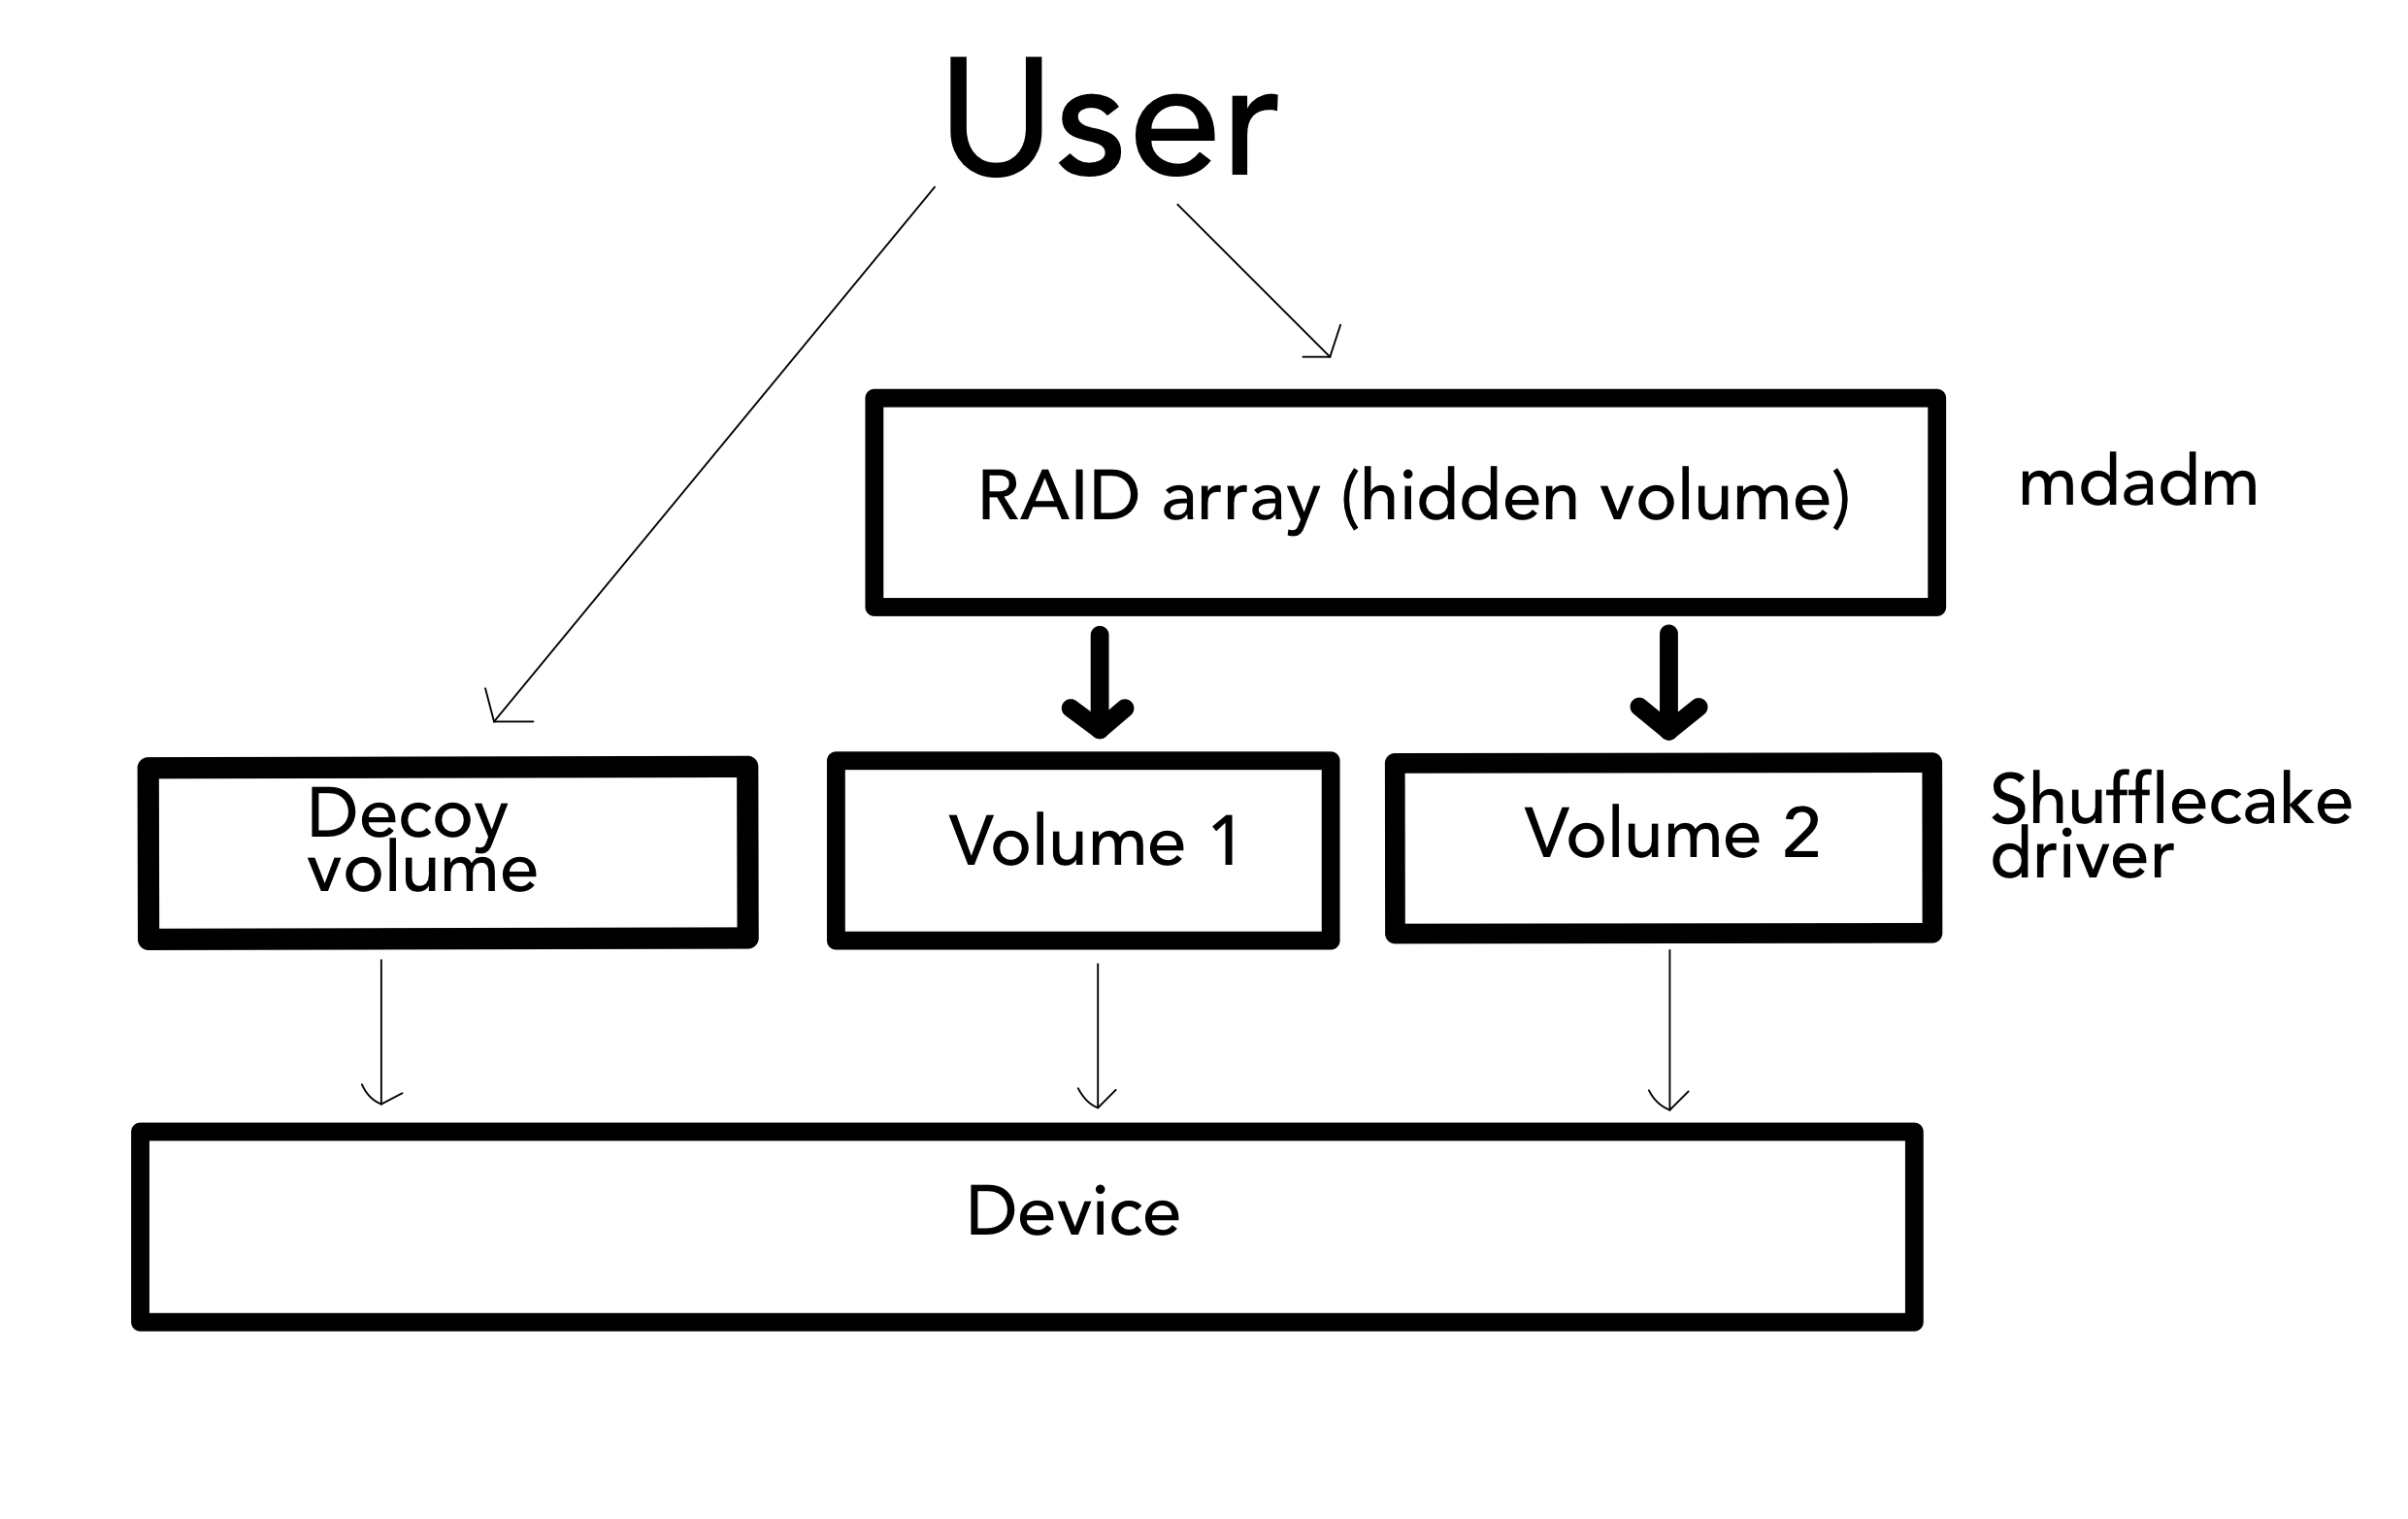
\includegraphics[width=0.8\textwidth]{Figures/red_mdadm.png}
\caption{mdadm redundancy layout}
\label{fig:red_mdadm}
\end{figure}

\subsection{Replication}

As previously stated, there is no need to add redundancy to the first Shufflecake volume that serves as a decoy volume. For the remaining volumes, we will need two Shufflecake volumes for each RAID array that will serve as hidden volume(s). Using mdadm, we create each array as follows:
\begin{verbatim}
    sudo mdadm --create --verbose $raid_array_path --level=1 --raid-devices=2
    $first_volume_path $second_volume_path
\end{verbatim}
Then, whenever we reopen the volumes, we reassemble each array:
\begin{verbatim}
    mdadm --assemble --update=resync $raid_array_path $first_volume_path
    $second_volume_path
\end{verbatim}
Where we resync the array each time we open it to ensure that any corruption is corrected before the RAID array is opened. Afterwards, it can be mounted and used just like any other block device. The regular Shufflecake block devices that make up the RAID array are still available, but they should not be used on their own. These commands can be easily automated when the volumes are created or opened.

Mdadm will handle the replication of data between the two mirrored volumes as well as the repair of any corruption using the mirrored data. However, as previously stated, this corruption occurs because multiple volumes are assigned to the same physical slice. If we begin the repair without fixing those inconsistencies, it could lead to even more corruption. To prevent it, before we begin the repair, we must resolve these inconsistencies within the Shufflecake driver.

\subsection{Repair}

We examine all slices of all available volumes as soon as they are opened, comparing slice mappings to see if physical slices were assigned to multiple volumes logical slices. We can accomplish this by utilizing a constructor callback function provided by the device mapper framework and already in use in the driver. This function is called whenever a volume is initialized from a userland application, but it is executed independently for each volume, so we cannot directly repair them. We need to save a reference for each volume that is opened, and then use those references to compare all slice mappings as the last one is opened.

Fortunately for us, because of the recursive hierarchy structure, volumes are always opened from most to least secret, and at least one volume has to be opened. That means that the primary decoy volume will always be opened and this is where we will do our consistency check.

We loop through all available volume pairs and compare their slice mappings for double allocations. If there is, as previously explained, we favor the least secret volume in the slice attribution and allocate a new slice for the other volume. If the mirrored version of this slice is still available, this newly allocated slice will be filled with its original content during the repair.

This repair operation is computationally demanding, with a complexity of \( O(n^2 * m^2) \), where n represents the number of volumes opened and m represents the total number of slices available in the underlying device. However, the actual repair cost is quite low because we only need to allocate a new slice. However, the resync operation performed by the RAID manager when we assemble the array takes a long time because the volumes are scanned again in their entirety. It is acceptable because the repair is only performed once at startup, but it is not ideal. After the repair, the references to the volumes can be erased.

Mdadm will attempt to find and open clusters automatically. We must avoid this behavior if we want to force the mirrored volumes to resync each time they are opened. Array auto-assembly can be disabled in the configuration file. Also, RAID1 does not provide any protection against silent data corruption. If some data on one of the mirrored volumes was altered but still readable, no correction would be triggered because there is no added integrity data and thus no way for the RAID manager to know which version is the correct version. This is not an issue in our case because the type of corruption we are attempting to repair will always be non-silent.

Unfortunately, the RAID manager only sees sectors on block devices and has no view on the slices. It is unable to optimize its mirroring, which causes some issues as we will see in the results. This approach was designed as an introductory experiment and was not fully integrated into the modified Shufflecake code.

\section{Redundancy among multiple volumes}

To better integrate with the Shufflecake slice system, we must create our own RAID-like solution that works directly at the driver level. It can then be optimized to work with slices and reduce the repair time. The volume layout will be similar to the previous approach in that the first volume serves as a decoy and is not redundant, and the subsequent volumes are paired to form hidden volumes. An example layout can be seen in figure \ref{fig:red_among}.

\begin{figure}[ht]
\centering
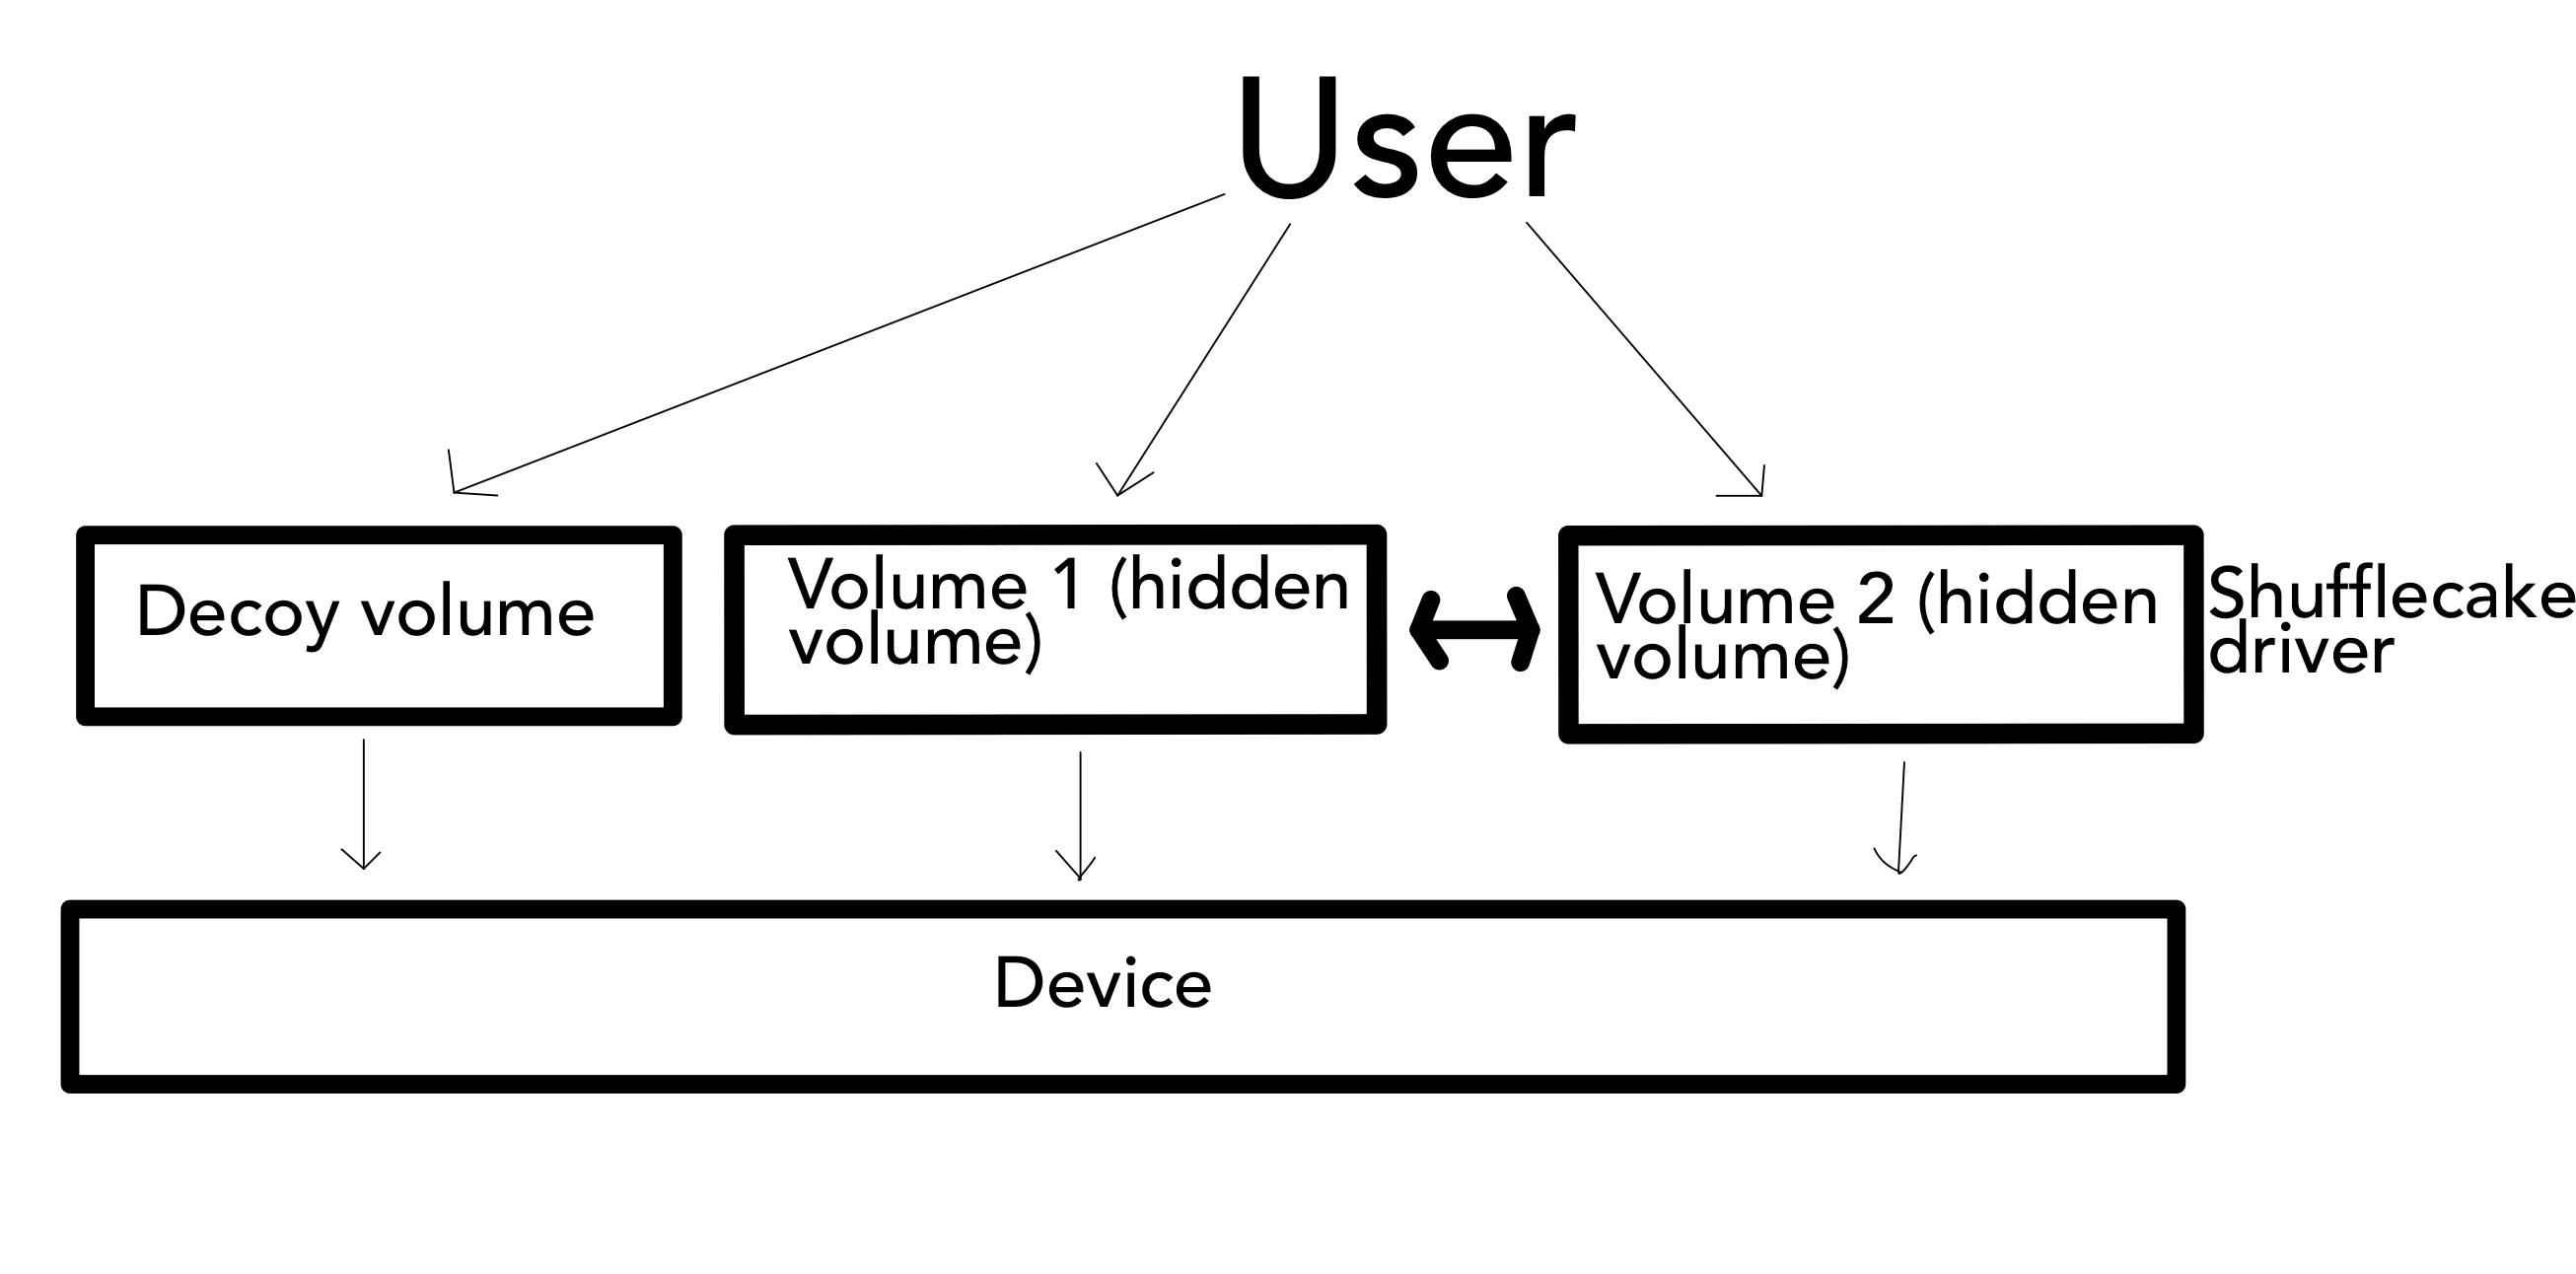
\includegraphics[width=0.8\textwidth]{Figures/red_among.png}
\caption{Layout of redundancy among multiple volumes}
\label{fig:red_among}
\end{figure}

\subsection{Replication}

To begin, we modify the driver in order to replicate the slice content between these volume pairs. We can use another device mapper framework callback, which is a mapping function that is called for each block I/O request sent to one of the volumes.

These block I/O requests are contained in basic containers known as bio. They represent in-flight block I/O operations, which are essentially reads or writes to volumes linked to memory pages. The device mapper framework allows us to intercept these objects and perform actions on them before submitting them to be processed. This property is used by the driver to transition from logical to physical space. Requests for logical slices are received in cleartext if they contain data (in the case of volume writes). They are converted to the correct physical slice using the volume slice mappings, and the pages are either encrypted before writing or decrypted after reading\cite{10.5555/1855096}.

When we receive write requests to one of the two volumes that make up a hidden volume, we want to send an identical request to the other volume in the pair. This ensures that all data is replicated between the two volumes. This intercepting function, like the previous contructor callback that we used in the repair, is called independently for each request of each volume, and we do not have direct access to the other volumes. Fortunately, the repair mechanism already generates a global list of references to the opened volumes. Because this procedure will be reused for this approach, we only need to keep this list instead of destroying it at the end of the repair. Finally, we can use another callback, the destructor callback, which is called for each volume when it is closed, to remove this list from memory.

The initial plan was to allocate a new bio request destined for the mirror volume and match its fields to the original one, along with all the other structures required. As it turns out, creating a correct request from scratch is difficult, and debugging them is very time-consuming. Most bugs cause kernel faults that are difficult to recover from; frequently, the only solution is to restart the machine. At this point, I switched my testing to a virtual machine, which made it easier to track down kernel errors and reboot faster when necessary. Ultimately, this led to other problems, which I will discuss later.

I also configured a debug kernel within the virtual environment and interfacing it with gdb\cite{VMGDB}, but it was difficult to use. It was far more efficient to simply print messages at the appropriate location into the kernel ring buffer and then display them with the dmesg command\cite{dmesg_man}.

At this point, I learned two critical pieces of information from the creator of Shufflecake, Elia Anzuoni, after some exchanges. For starters, block I/O requests cloned from other requests do not own their memory pages. Second, all requests that arrive at the mapping callback are already cloned requests. If we follow one of them, we can see that in the case of a read, a shallow copy of the original request is made in order to transition it to physical space. Only the copy is submitted in this case because the pages are decrypted in place, so there is no need to own them; it is simply another clone, like we can see in figure \ref{fig:bio_read}. However, for a write, we must encrypt the pages before sending them to the device, and we must own the pages in order to do so. As a result, a deep copy is created and then submitted.

Nothing prevents us from making another clone of the block I/O request received from the device mapper framework and forwarding it to the mirrored volume because it is already a clone of the original. During the write operation, each of the two requests will have its own deep copy so they will not interfere with each other. This ensures that the paired volumes stay identical in logical space even if they are physically independent and different, like we can see in figure \ref{fig:bio_write}.

\begin{figure}[ht]
     \centering
     \begin{subfigure}[b]{0.49\textwidth}
         \centering
         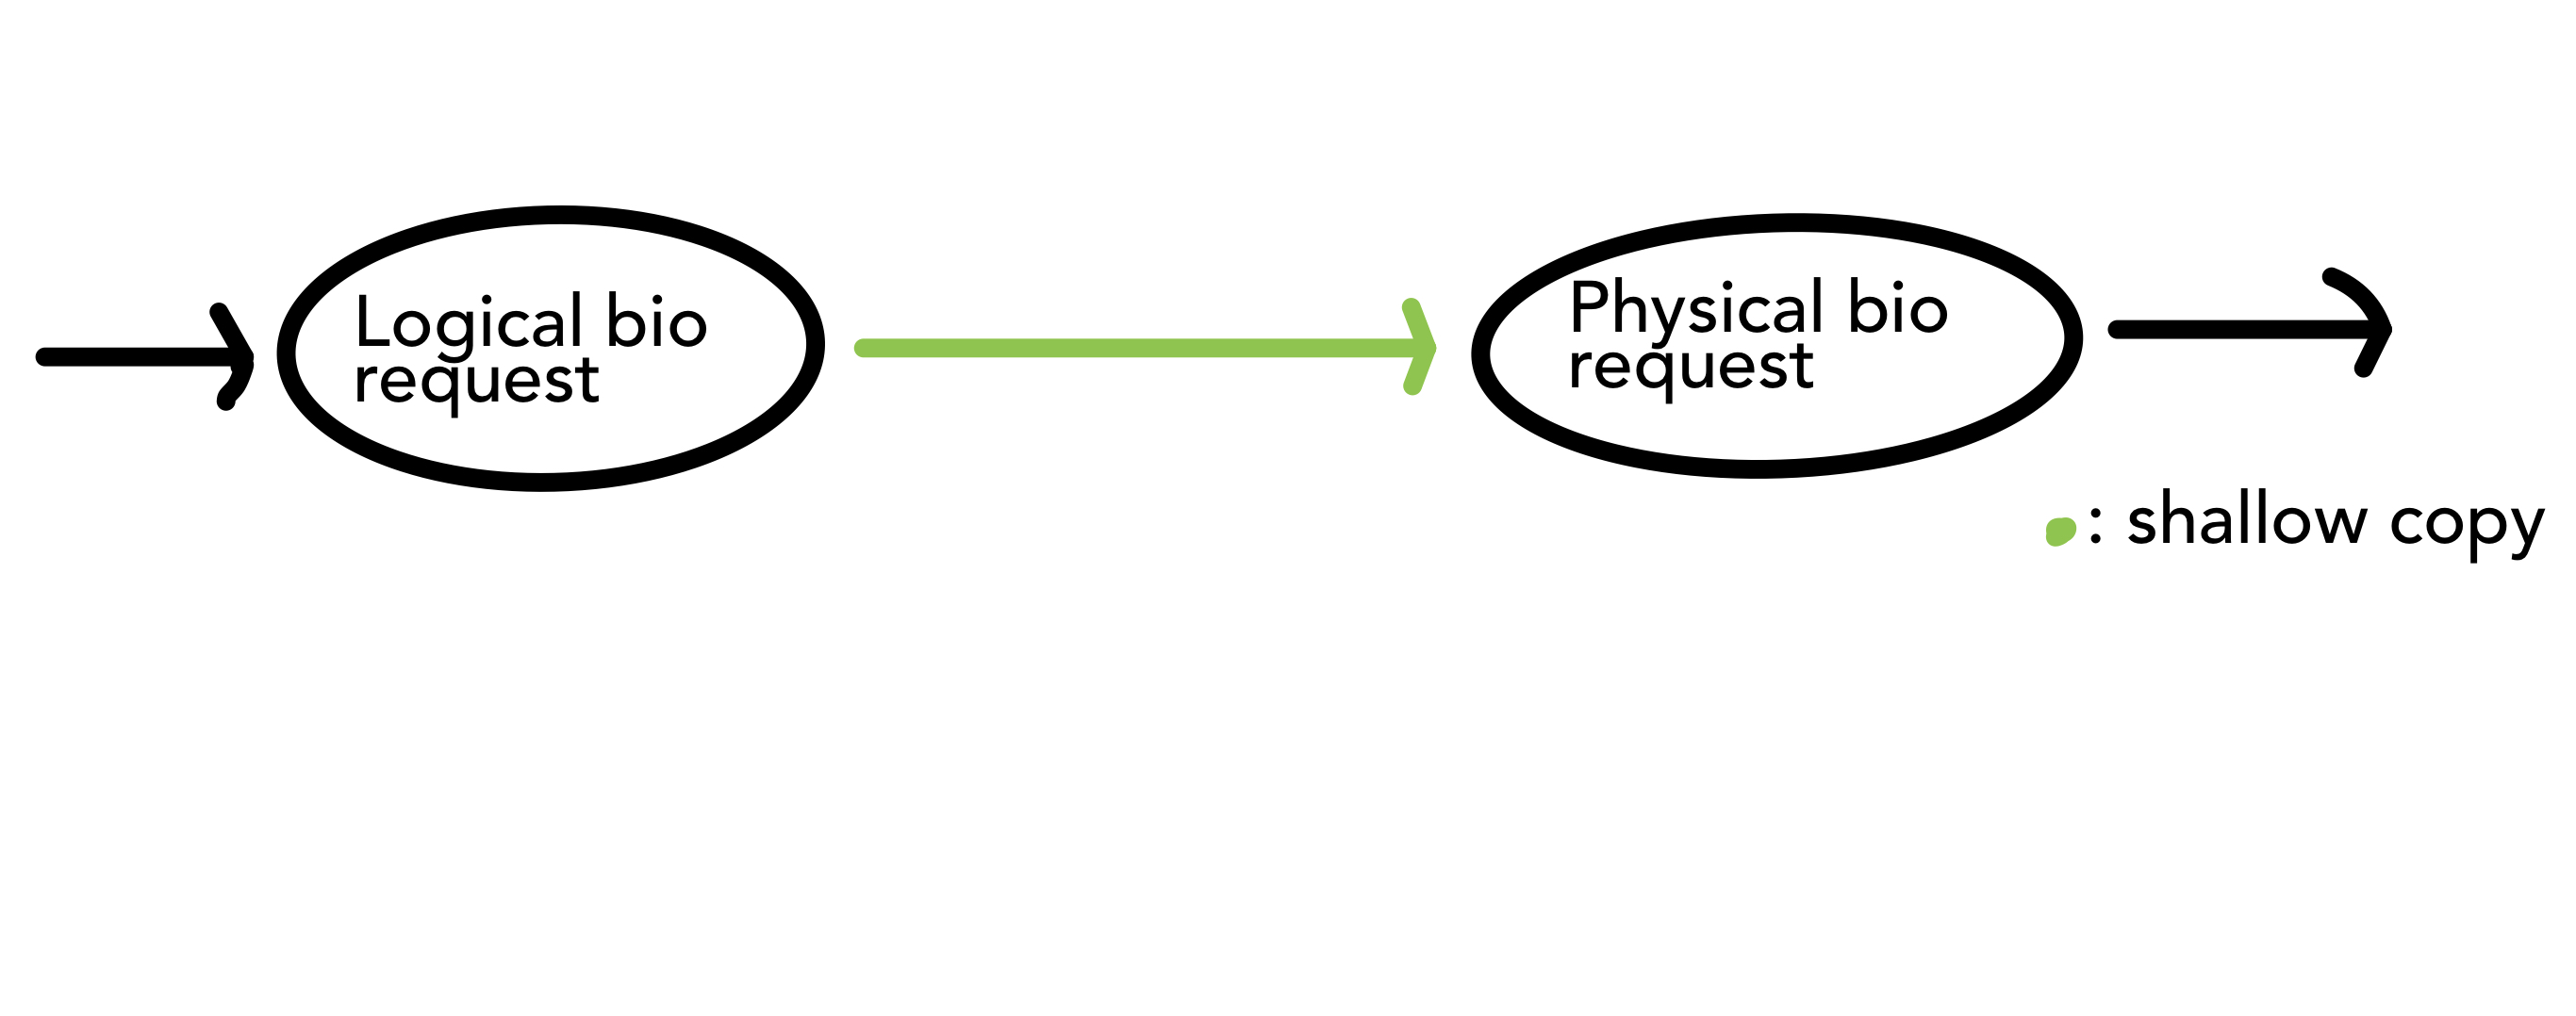
\includegraphics[width=\textwidth]{Figures/bio_read.png}
         \caption{READ}
         \label{fig:bio_read}
     \end{subfigure}
     \hfill
     \begin{subfigure}[b]{0.49\textwidth}
         \centering
         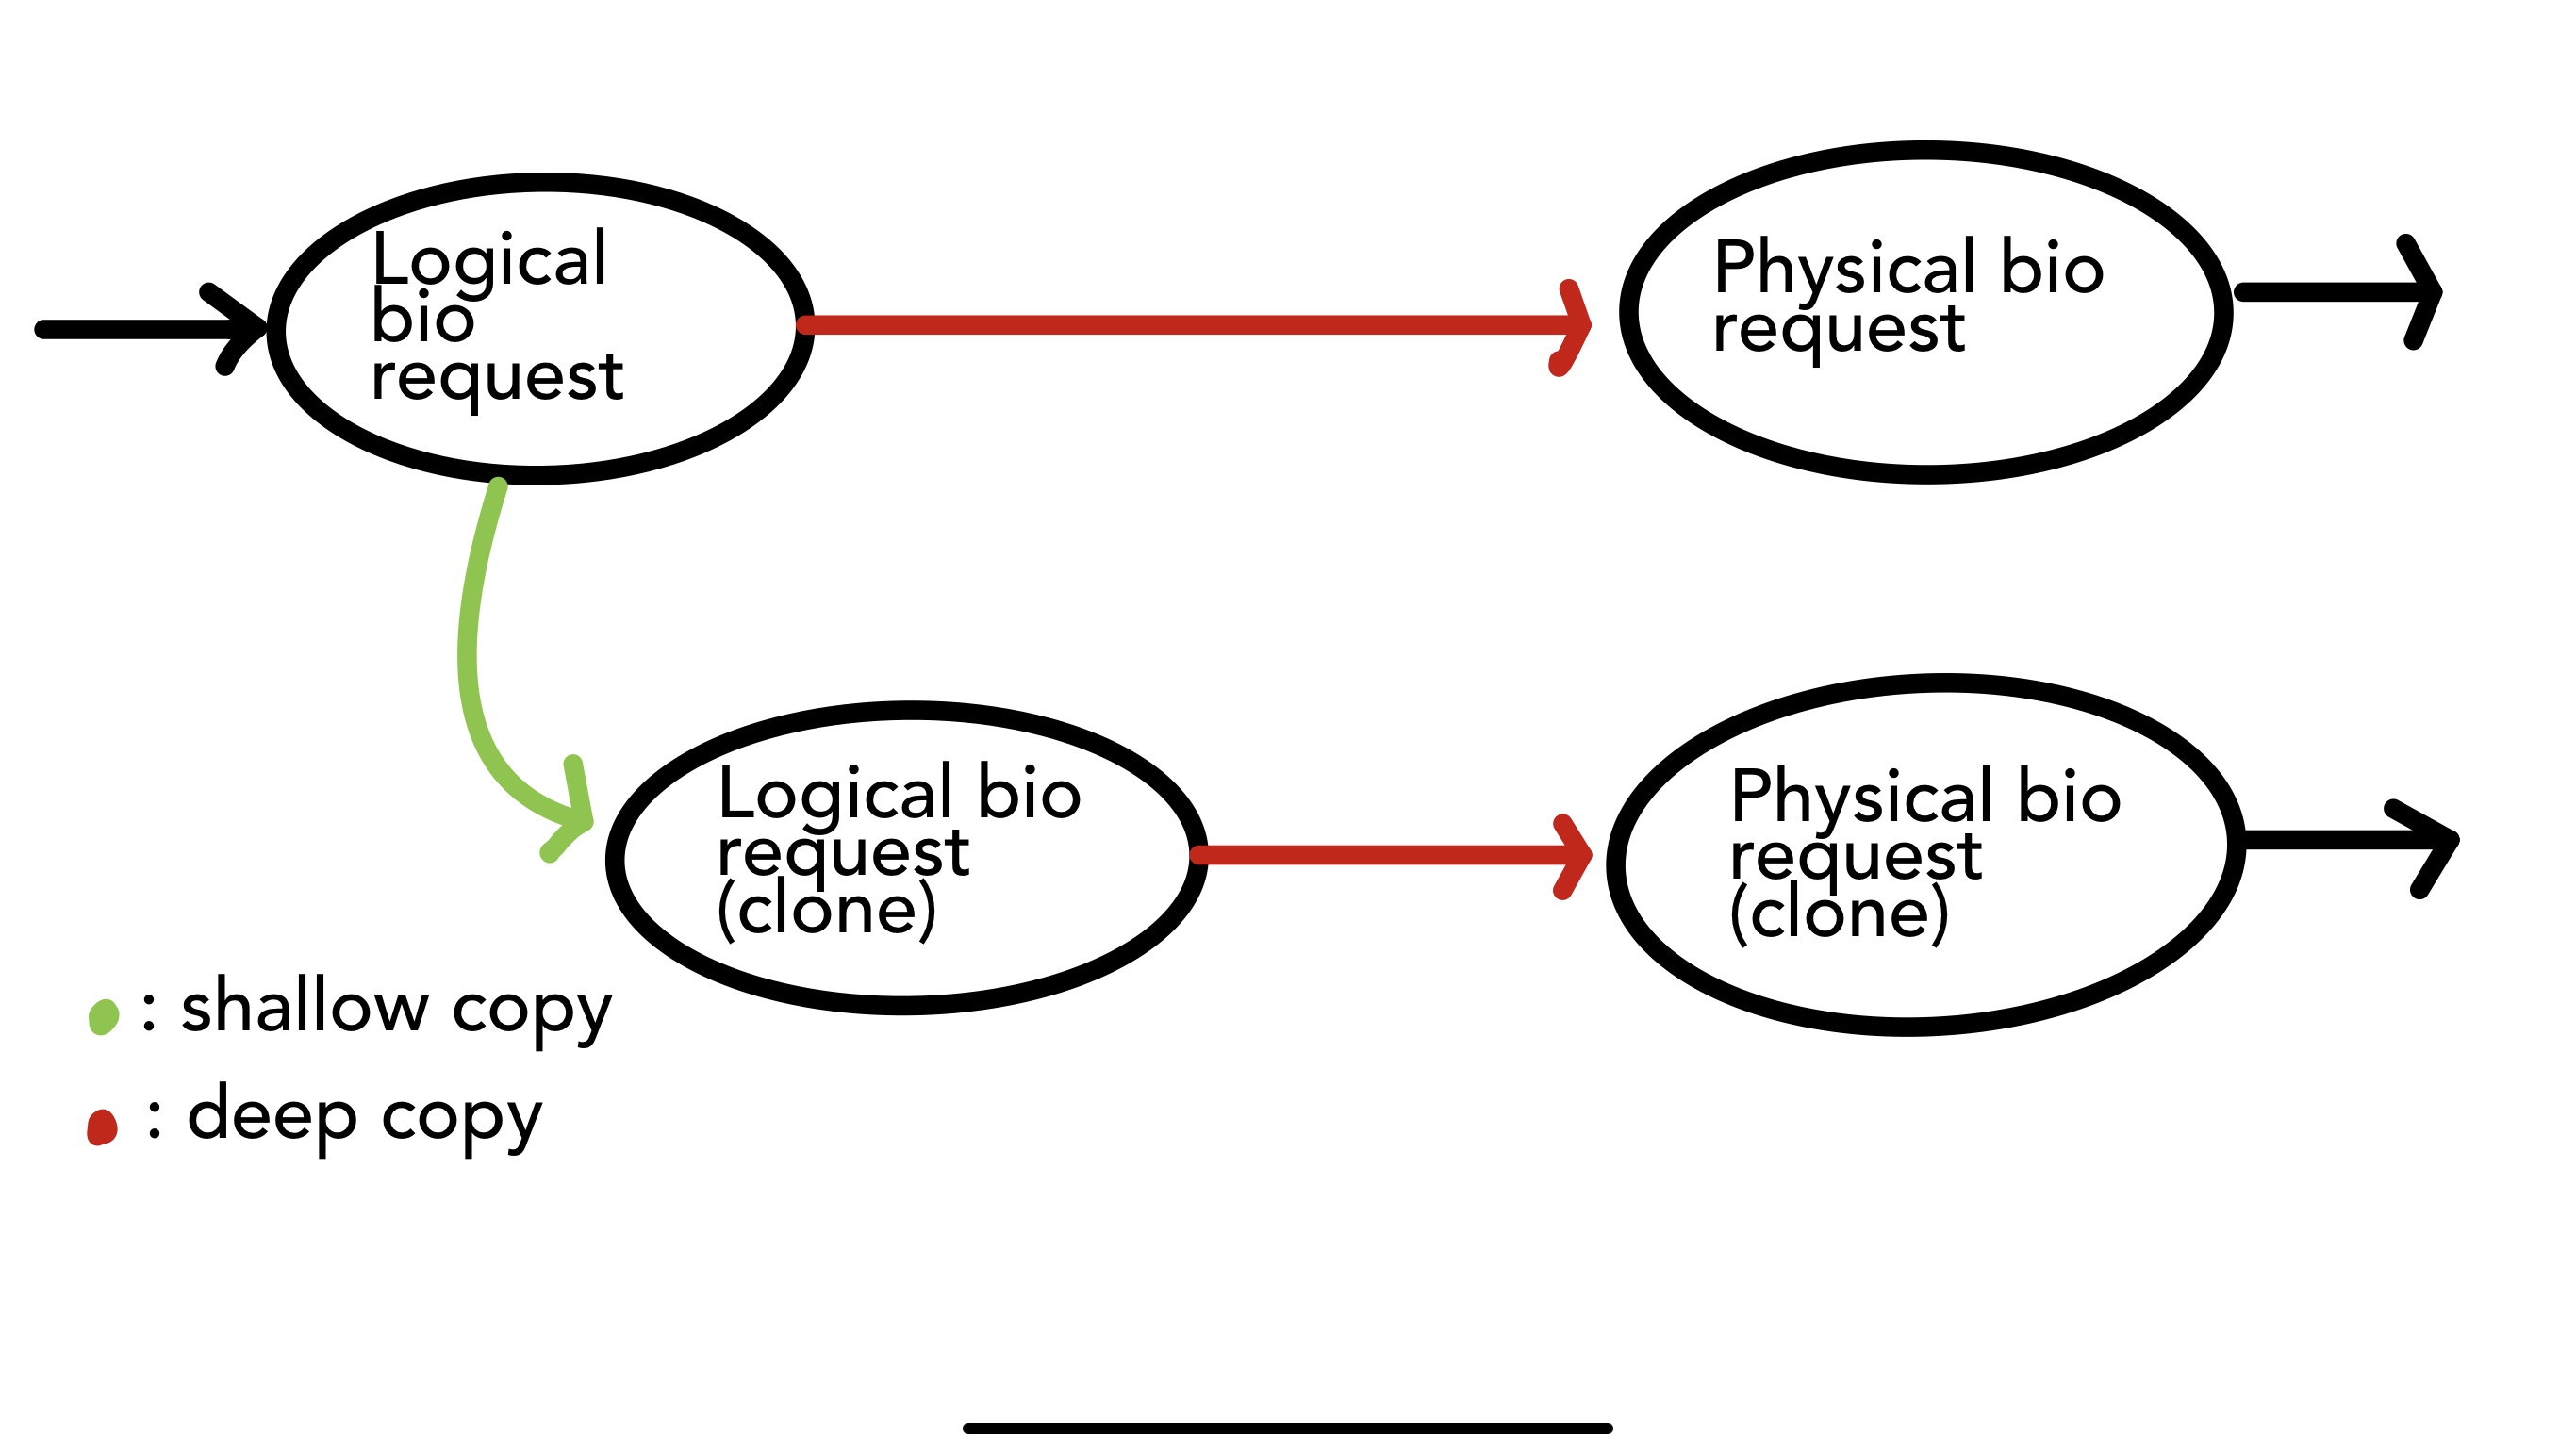
\includegraphics[width=\textwidth]{Figures/bio_write.png}
         \caption{WRITE}
         \label{fig:bio_write}
     \end{subfigure}
        \caption{Processing of bio requests}
        \label{fig:bio_process}
\end{figure}

\subsection{Repair}

To disambiguate the slices, we can reuse and improve on the repair mechanism developed for the mdadm approach and extend it. When an inconsistency is detected, we not only allocate a new slice but also copy the content of the "backup" slice on the other volume into this new slice.

The Shufflecake code includes a function that allows us to read and write blocks to the device directly. However, the data is manipulated in its encrypted form. We must read the data blocks of the slice from the non-corrupted volume of the pair, that we will call the donor volume, decrypt it, re-encrypt it, and write it to the corrupted volume, that we will call the receiver volume. The cryptographic operations are performed using the cryptographic contexts of the volumes in question. We can access them via the list of volume references created when the volumes are opened.

We also need the initialization vectors for the decryption and encryption of the data blocks. One physical slice is made up of 256 data blocks, and all of their IVs are stored in a single additional block at the beginning of the physical slice. The slice mappings can be used to find the starting blocks of the physical slices in both volumes. The index of the slice times the block size of a physical slice will be the block location in the data section. To this number, we have to add the size in blocks of the header section that precedes the data section.

The complete procedure, that we will call a slice transfusion is pretty straightforward :
\begin{enumerate}
    \item Compute the starting sectors of the physical slice on the donor and receiver volume.
    \item Read the IV block on each volume.
    \item For the 256 following data blocks :
    \begin{enumerate}
        \item Read and decrypt the data block from the donor volume using its IV.
        \item Encrypt and write the data block to the receiver volume using its IV.
    \end{enumerate}
\end{enumerate}
To prevent any changes, the slice mappings of the affected volumes, as well as the device reverse mapping (used to find available slices), are locked during the slice transfusion.

We loop through the volumes and their respective slice mappings but we cannot simply fix corruption as we go. We do not want to repair a slice with its backup data only to discover later that the backup data was also corrupted. We need to detect those double corruptions and skip the slice transfusion on them.

A first pass is done to detect slice inconsistencies and store their locations in a list of specialized structures. We then go through this list to correct any inconsistencies and only perform the transfusion from a donor to a receiver if the donor was not also corrupted. In the case of a double corruption, the lost data is unrecoverable anyways so the space will be reused as needed in the future.

Because the number of slice inconsistencies is often much smaller than the total number of slices, the cost is absorbed and the complexity is similar to the previous approach. The actual repair cost is higher because a transfusion may be required, but it is faster than rescanning the entire drive to resync the RAID array. Overall, this method speeds up the repair process.

The volumes can be used normally once the repair is completed. Because of the replication, either volume of the hidden volume pairs can be used. The data will simply be replicated on the second one. To improve usability, one block device in each pair forming a hidden volume should be rendered invisible to the user or made inaccessible. We could not figure out how to do it without heavily involving the operating system, so the idea was dropped.

\subsection{Implementation}

This mitigation is included in the modified version of the Shufflecake available on the project repository\cite{github}. The volumes can be opened in this redundancy mode by passing the \verb|--redundant-among| parameter to the open command, activating the replication and repair.

Ideally, the command used to create the volumes would also have been modified, so that each password given to create a hidden volume would directly create a pair of volumes. As we only provide one password, we could either use the same password for both volumes of the pair, or we could give the password to the volume of the pair highest in the hierarchy and use a random one for the other.

If multiple volumes have the same password, Shufflecake will open the volume at the top of the hierarchy first, and then the others recursively. As a result, using the same password on two volumes is possible. However, this behavior is subject to change, and we do not want to rely on it.

We prefer the alternative proposal of generating a random password for the other volume. We do not need the user to know this extra password because we do not want them to be able to open only one volume of the pair. This ensures that the only way to open the second volume of the pair is through recursion, and that this recursion will always occur when we open the first. Hence, both volumes will always be opened together.

Due to time constraints, this modified creation of volume could not be implemented in the code.

\section{Redundancy within volumes}

Designing a redundancy that works across multiple volumes was simple, thanks to the many similarities with RAID. However, it is not the best compromise for Shufflecake because it requires multiple volumes to achieve it. In the philosophy of Shufflecake, each volume represents a level of secrecy and security and we are violating this principle by pairing them. We can modify the solution slightly to maintain this proposition and keep the volumes separate.

It makes no difference whether we store our mirrored copies on the same or a different volume because the corruption rate is probabilistic and the volumes previously used in the pairs that made up the hidden volumes are always opened together. There are no additional space constraints because each Shufflecake volume can handle the entire storage capacity of the underlying device. This idea is showcased in figure \ref{fig:red_within}.

\begin{figure}[ht]
\centering
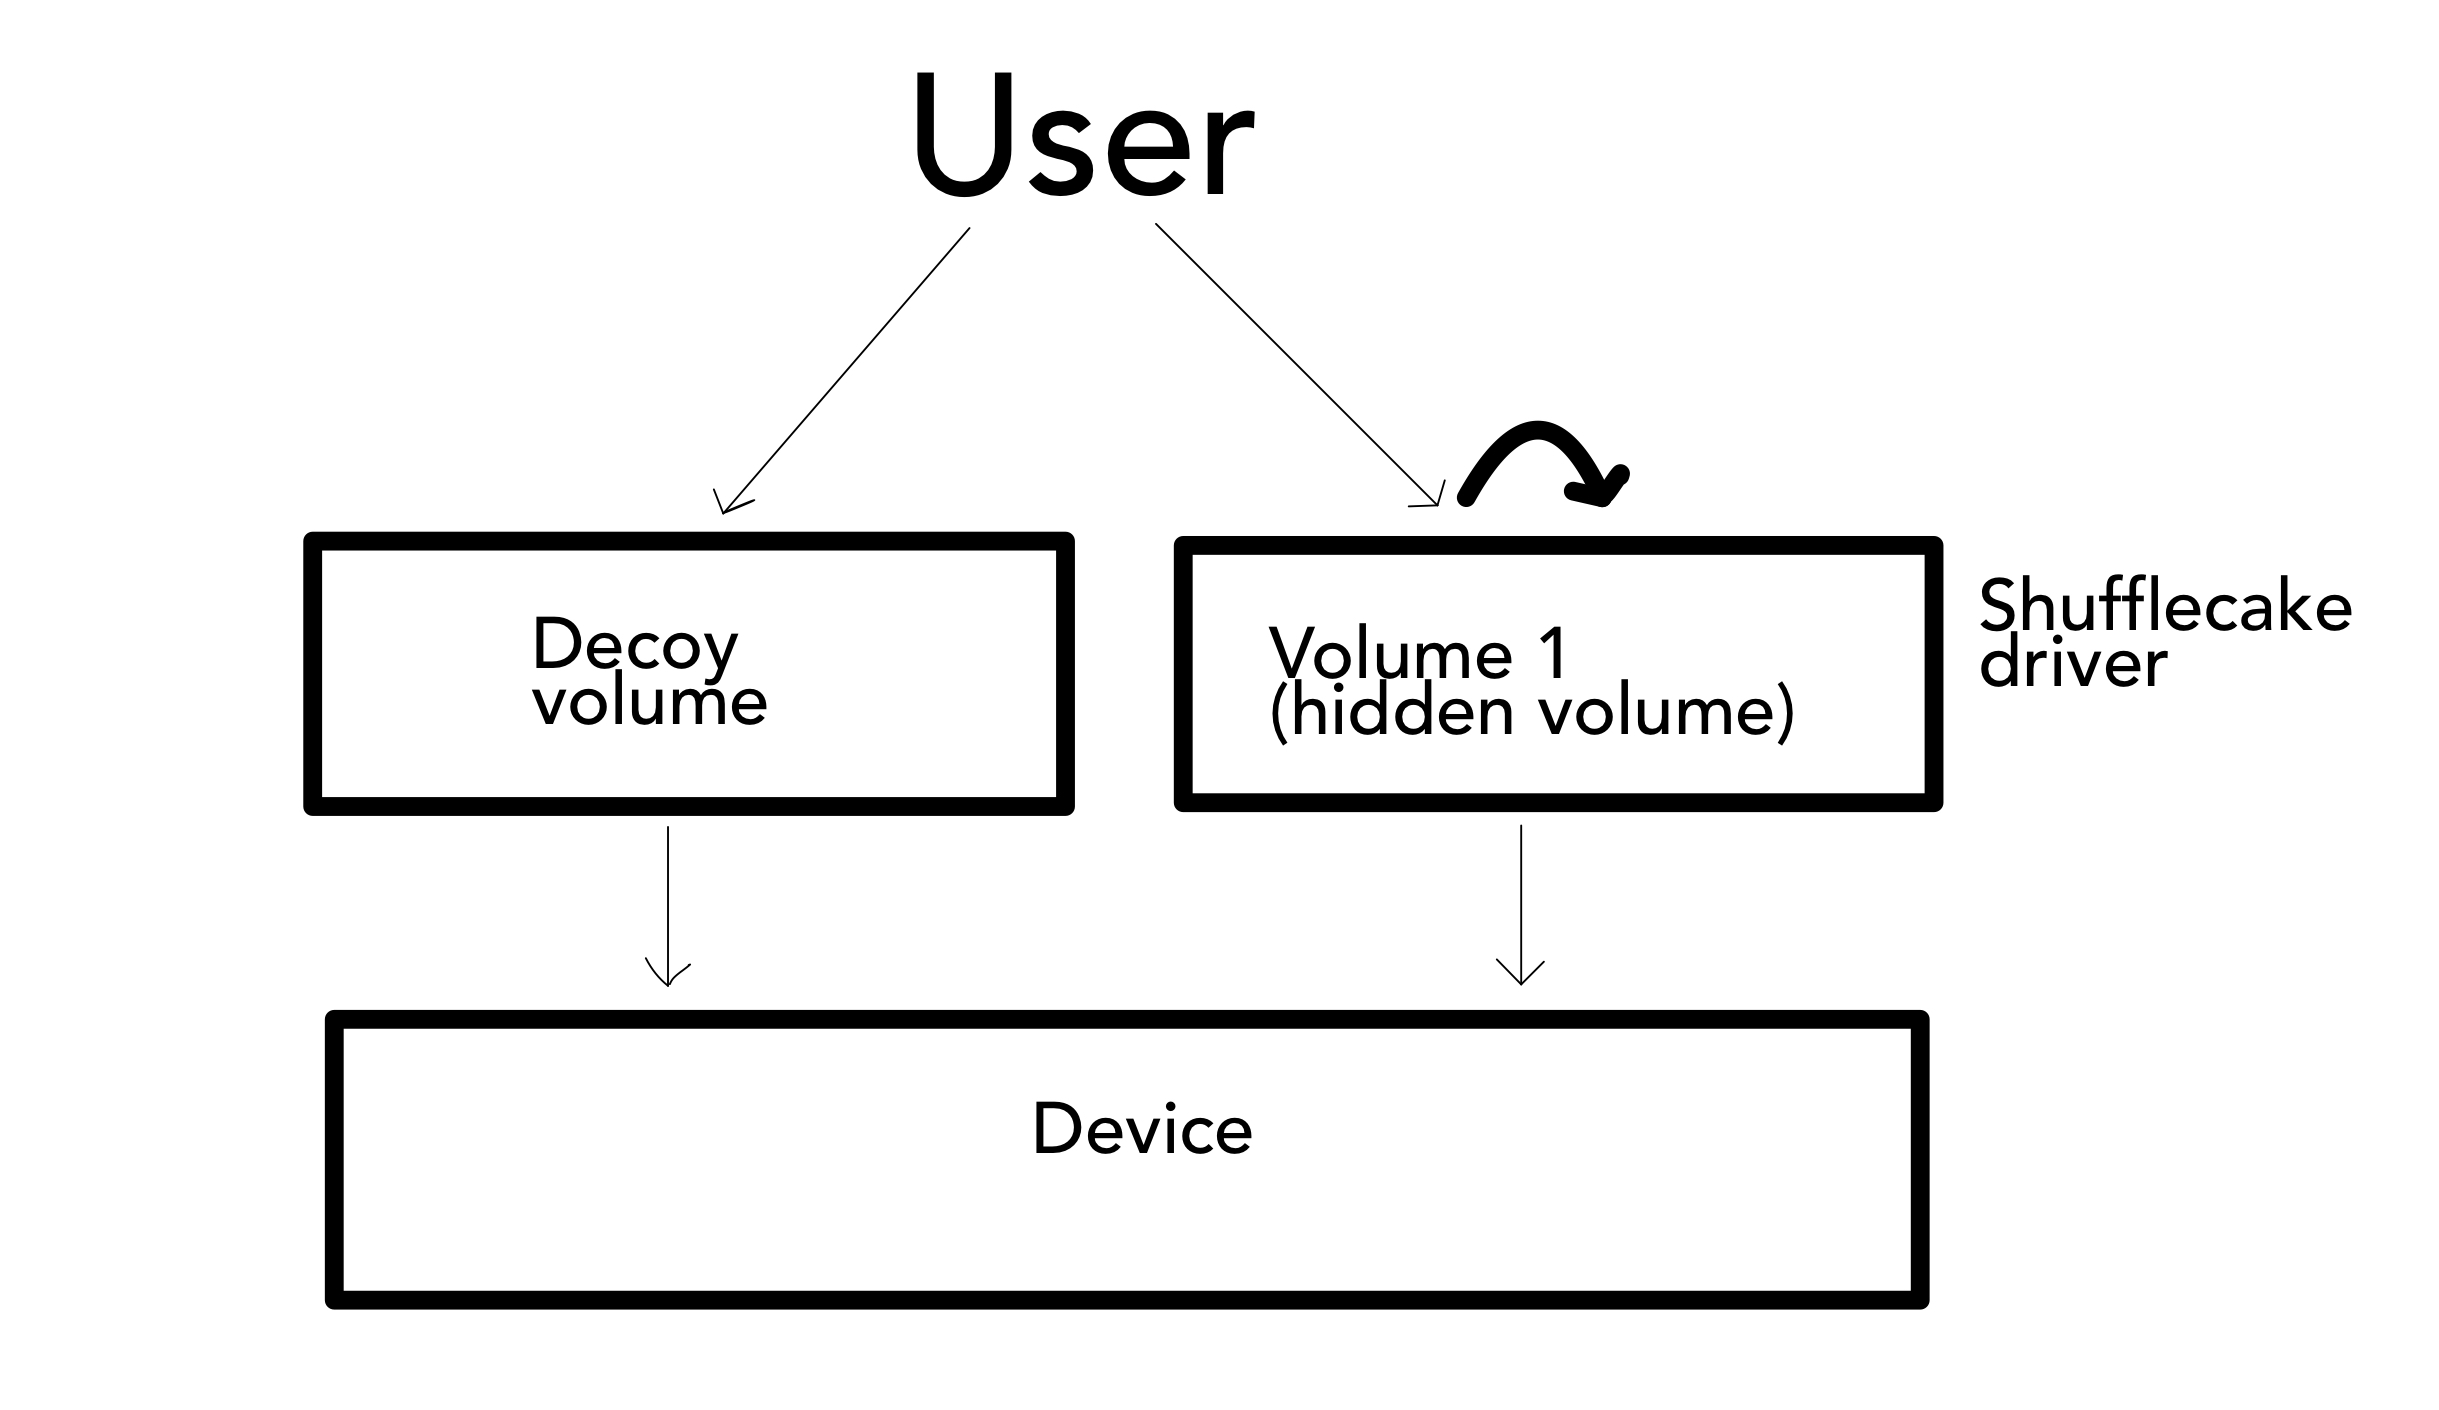
\includegraphics[width=0.8\textwidth]{Figures/red_within.png}
\caption{Layout of redundancy within volumes}
\label{fig:red_within}
\end{figure}

\subsection{Replication}

The callback function that we used for replication in the previous approach needs to be slightly tweaked. We will divide the volume logical space into two by selecting odd and even slices. Each odd logical slice will be paired with the even logical slice that comes after it. When we intercept a write request aimed at one of them, we forward it to the other in the same manner as before, but this time within the same volume.

It should be noted that, even if the paired slices are contiguous in the logical space, their respective physical slices may be in vastly different locations due to the random assignment. For this method to work, the total number of slices must be even; otherwise, one will not have a mirrored copy. To ensure this, we manually restrict the use of the last slice if the total number of slices available on the device is odd. While not the ideal solution, it is the most practical.

\subsection{Repair and implementation}

The repair is almost identical to the previous approach except that in the transfusion the donor and receiver are the same volume.

This mitigation was also included in the modified version of the Shufflecake available on the project repository\cite{github}. It can be enabled using the parameter \verb|--redundant-within| in the command to open the volumes, activating the replication and repair.

\newpage
\let\clearpage\relax

%%%%%%%%%%%%%%%%%%%%
\chapter{Results}
%%%%%%%%%%%%%%%%%%%%

\section{MDADM approach}

This method was the simplest to implement. Corruption is successfully dealt with and the files are kept consistent and protected. However, because the RAID manager cannot see the slices, this results in wasteful use of them and by extension of the storage space. We noticed that it was using far too many during the repair phase. There is currently no garbage collection implemented for the slices within Shufflecake, and they cannot be reclaimed once assigned. This renders this approach unusable for the time being, as we run out of slices far too quickly.

It has, however, a good usability because we only need to manipulate the RAID block device without having to worry about the underlying layout (even though the block devices that make up the array are still visible to the user). Because each RAID array contains two Shufflecake volumes, the total number of volumes is reduced to seven hidden arrays on top of the primary decoy.

The mdadm solution was not tested or developed further, but it would be a good approach to come back to if Shufflecake were to implement garbage collection in the future.

\section{Redundancy among multiple volumes}

We tried another solution that required working deep within the system and on drivers, which proved to be far more difficult than anticipated. Simple errors frequently resulted in system-wide crashes. This necessitated the use of a virtual machine during testing, which had its own set of issues. The USB driver would occasionally hang and stop responding due to some strange interaction between this kernel version and the virtual environment. It was difficult to distinguish between problems caused by the VM and those caused by the code itself, which made progress slow and tedious.

This approach does not work perfectly at the moment due to all of these obstacles. When corruption occurs, most slices are replicated and repaired, but some sectors still cause faults during this process. We were able to isolate at least some of the blocks causing issues in the current testing scenarios. The culprits appear to be, at least in part, the filesystem superblocks and their copies. When they are processed, they cause general protection faults that are extremely difficult to recover from and almost always necessitate a machine reboot.

When we stop implementing redundancy for these specific blocks, the mitigation works. However, because the superblocks are not protected against corruption, the volumes remain extremely unstable, making thorough testing impossible. As soon as the superblocks gets corrupted, the filesystem crumbles. Because the location of the superblocks is determined by the size of the device storage space, this dirty fix is heavily tailored for our current testing scenario and will not work elsewhere. We can, however, demonstrate the effectiveness of the mitigation on a single testing run that did not suffer from superblock corruption for many rounds.

\begin{figure}[ht]
     \centering
     \begin{subfigure}[b]{0.3\textwidth}
         \centering
         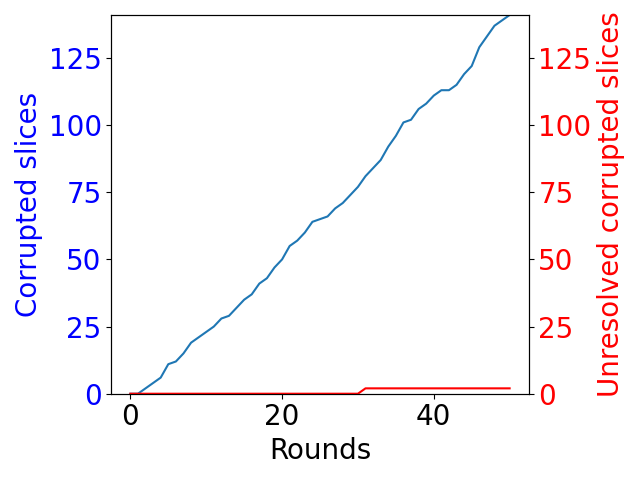
\includegraphics[width=\textwidth]{Figures/mitigated_corruption_rate_300KB.png}
         \caption{Light workload}
         \label{fig:among_mitigated_slice_light}
     \end{subfigure}
     \hfill
     \begin{subfigure}[b]{0.3\textwidth}
         \centering
         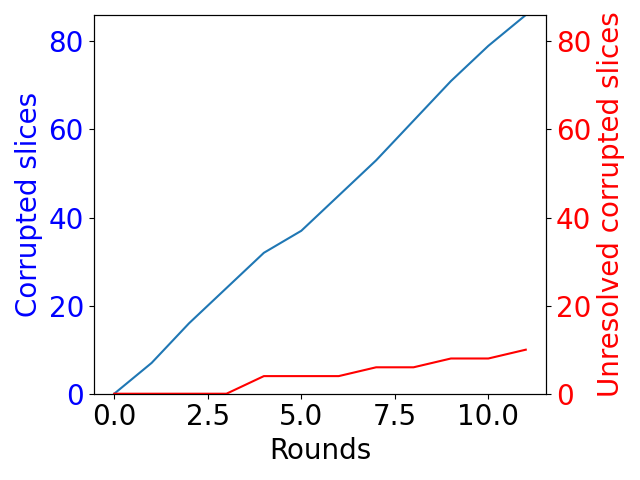
\includegraphics[width=\textwidth]{Figures/mitigated_corruption_rate_1MB.png}
         \caption{Medium workload}
         \label{fig:among_mitigated_slice_medium}
     \end{subfigure}
     \hfill
     \begin{subfigure}[b]{0.3\textwidth}
         \centering
         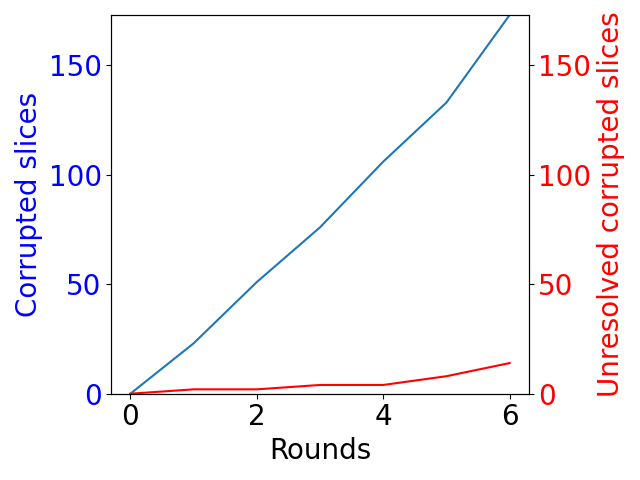
\includegraphics[width=\textwidth]{Figures/mitigated_corruption_rate_3MB.png}
         \caption{Heavy workload}
         \label{fig:among_mitigated_slice_heavy}
     \end{subfigure}
        \caption{Slice corruption analysis with redundancy among multiple volumes}
        \label{fig:among_mitigated_slice_analysis}
\end{figure}

We used the same testing settings as for the previous tests on slice corruption to be able to easily compare the results. In figure \ref{fig:among_mitigated_slice_analysis}, we plotted in blue the amount of corrupted slices that are detected and in red those that remain corrupted after the repair. As we can see the results are really encouraging with 88 to 98\% repair efficiency. The slices that cannot be repaired are the ones that got "double-corrupted". We can observe that we get more of them in heavier workloads as we have a lot more corruption to repair at once, and so a lot more probability to have a slice and its mirror be corrupted at the same time. We deduce that the other variations are due to random fluctuations as we could not repeat the test many times to get an average. 

Because the user has access to both volumes in the pair forming the hidden volume, the usability of this approach is not ideal. We can work on either of them, but one should be hidden from view for convenience. As previously stated, we were unable to accomplish this without heavily involving the operating system so the idea was dropped. Like the mdadm method, it also cuts the maximum number of hidden volumes in half.

\section{Redundancy within volumes}

The last solution shares many similarities with the previous one, as well as many of its setbacks. We could not manage to test the rate of corruption in this implementation as it was too unstable. Many blocks trigger faults when accessed and, unlike previously, we could not pinpoint the cause nor isolate these blocks. 

We think that the problem still relies in the integration of the filesystem to the system. However, we suspect that there is more at play than simply the superblocks this time. It seems like the filesystem does not handle very well the separation of the storage space by splitting even and odd slices. It wants to place data at specific locations but it is not always possible as we restrict some of the space to use in our mirroring. To verify this hypothesis, we would require additional testing that could not be done due to time constraints.

If we can get it to work, this approach is overall a better option. It has a better usability because it works exactly like plain Shufflecake, without any added constraints, and it adheres to the tool's original philosophy. The number of hidden volumes is also not reduced unlike the other approaches.

\section{Comparison}

Using the fio benchmarking tool\cite{fio}, we evaluated the performance of the various mitigations. We ran the test in a similar setting to what was used before, utilizing a 1GB USB stick with USB 3.0. We ran the tests on both a physical and virtual machine running Ubuntu 22.04 with the 5.15 Linux kernel on an Intel Core i7. Standard workloads of sequential and random reads and writes were performed. The overhead is measured in comparison to a baseline installation of Shufflecake version 0.1. Table \ref{tab:results} shows the difference in performance.

\begin{table}[ht]
\begin{center}
\begin{tabular}{ |c||c|c|c|c|  }
 \hline
 \multicolumn{5}{|c|}{VirtualBox VM} \\
 \hline
 & Shufflecake & mdadm & Among & Within\\
 \hline
 Seq. Reads & 112 & 53.6 & 104 & 81.8\\
 Seq. Writes & 4.35 & 1.66 & 0.89 & 0.85\\
 Rand. Reads & 68.4 & 24.8 & 88 & 77.8\\
 Rand. Writes & 2.6 & 0.62 & 0.77 & 0.72\\
 \hline
 \multicolumn{5}{|c|}{Native machine} \\
 \hline
 & Shufflecake & mdadm & Among & Within\\
 \hline
 Seq. Reads & 238 & 223 & 255 & 225\\
 Seq. Writes & 7.8 & 2.86 & 1.43 & 1.38\\
 Rand. Reads & 180 & 96.9 & 236 & 227\\
 Rand. Writes & 5.84 & 1.26 & 1.29 & 1\\
 \hline
\end{tabular}
\caption{Measured throughputs (in MiB/s)}
\label{tab:results}
\end{center}
\end{table}

We can see that the performance on the native machine is higher in absolute terms, despite both being very similar in relative terms. The minor differences can be attributed to fluctuations in the benchmarking process.

When compared to plain Shufflecake, the mdadm approach has a performance overhead of 1-3x for reads and 2-5x for writes. We attribute the slowdown to the additional layer added by the RAID manager that the data has to go through. For the other two implementations, we can see that the performance overhead is very similar for both redundancy among multiple volumes and within volume, with no overhead for reads and a 3-6x overhead for writes compared to the baseline. The results line up with our expectations. We did not modify the processing of the read requests so no change is expected here compared to the baseline. We can see that the writes results are close to the mdadm ones in terms of performance and we could probably get them even closer by optimizing the request processing code.

We are not measuring the speed difference in the repair process for two reasons. First, the performance of the repair is is not critical because it only occurs once as the volumes are opened. Second, it would difficult to measure and compare it reliably as we cannot predict the corruption before it happens. However, as previously stated, we noticed that the repair process was faster in our two custom redundancy implementations than when using mdadm. This is most likely due to the fact that we are only scanning the entire volumes once instead of twice.

In the mirroring process, we use 1-to-1 copies of all data. As a result, all hidden volumes have a 2x storage overhead. Switching to another redundancy scheme, equivalent for example to RAID5 or RAID6, could improve space utilization. Additionally, this mirroring could be replaced by open or closed entanglements to increase the reliability\cite{entanglements}.

When redundancy is applied within volumes, the storage overhead is slightly higher because we may have to discard one of the slice of the device to keep their number even. The additional waste of space is minimal. This space, however, could be used for other purposes, such as keeping track of the corruption. Of course, this corruption journal would have to be concealed during normal operation and only made available when, for example, all volumes are unlocked as well to maintain the PD guarantees.

Ultimately, all mitigations implemented rely on the Shufflecake software security guarantees and do not expand on them. However, as previously stated, shifting the burden of responsibility to the user may be problematic for those who are unfamiliar with operational security. We acknowledge that these mitigations might not be appropriate in all situations.

\section{Shufflecake update}

Shufflecake received an update during the semester. We stayed on the older version for the rest of the project because it was already well underway and a lot of testing and code were designed for the original version. However, despite a thorough rewrite of the software, including extensive refactoring and bug fixes, nothing in the changes implies that the implemented mitigations would not work on the updated version with small adjustments.

\let\clearpage\relax

%%%%%%%%%%%%%%%%%%%%%%
\chapter{Conclusion}
%%%%%%%%%%%%%%%%%%%%%%

In the context of data storage, plausible deniability is a powerful concept. However, the concept of corruption resilience has received little attention in the PD security landscape. We investigated during this project Okhow to integrate it into existing tools, focusing on the Shufflecake software solution which allows us to create multiple hidden volumes with increasing levels of secrecy. We concentrated on the corruption caused by using the storage device while some of its sensitive data was hidden. Because the PD security guarantees make it impossible to prevent this corruption, we decided to focus on the recovery by implementing data redundancy.

We began by analyzing the rate of this corruption, then explored various levels of storage conceptualization before settling on one that met our testing requirements. We devised mitigations to reduce the rate of corruption, beginning with one based on existing software solutions and progressing to others that were more tightly integrated with the system. They work on a similar principle to RAID1 mirroring in that we keep 1-to-1 copies of the data at all times and use those copies to restore the corrupted sections.

During this project, we faced numerous challenges, the most significant of which were determining the level at which redundancy should be applied and interacting with the filesystem. To get usable results, we had to repeat our analysis on multiple storage unit levels, but in the end, all of the research and testing proved to be very useful when it came to designing the mitigations. Working with the filesystem was the most difficult aspect of this project. Many unanticipated complications arose as a result of its intricate nature and complex inner workings.

We could not bring this project to the point that we wanted to. We designed three different redundancy schemes and implemented two in the Shufflecake tool. However, they still suffer from usability problems that prevent us from thoroughly testing them, which explains the lack of consequent results. We could nevertheless produce promising findings and show the potential of such approaches in dealing with corruption in PD storage.

Further investigation into the usability issues could be conducted to identify the dependencies to the filesystem that hindered progress and understand how to overcome them. Additionally, exploring alternative redundancy schemes or refining the existing ones could help address the limitations encountered during the implementation phase.

\section{Further ideas}

The original Shufflecake paper investigates some methods for extending security guarantees against multi-snapshot adversaries, such as the inclusion of "ghost filesystems"\cite{Anzuoni:297353}. The goal of which is to make it appear as if there are always the maximum number of volumes used and to drown the signals of hidden volumes in noise. Shufflecake could support hidden operating systems stored on its hidden volumes to prevent information leakage caused by the OS. We would be interested to see how redundancies can be implemented and how current mitigations perform under these new constraints.

In terms of corruption resilience, there is no need for redundancy to only be kept local, and we could easily imagine copies being distributed across multiple systems. After being corrupted, those systems could repair each other. We believe that this is an intriguing approach to pursue, particularly in the context of decentralized and distributed systems.

\newpage
\cleardoublepage
\phantomsection
\addcontentsline{toc}{chapter}{Bibliography}
\printbibliography

\newpage

% Appendices are optional
%\appendix
% %%%%%%%%%%%%%%%%%%%%%%%%%%%%%%%%%%%%%%
% \chapter{How to make a transmogrifier}
% %%%%%%%%%%%%%%%%%%%%%%%%%%%%%%%%%%%%%%
%
% In case you ever need an (optional) appendix.
%
% You need the following items:
% \begin{itemize}
% \item A box
% \item Crayons
% \item A self-aware 5-year old
% \end{itemize}

\end{document}